\documentclass[conference]{IEEEtran}
\IEEEoverridecommandlockouts

\usepackage{cite}
\usepackage{amsmath,amssymb,amsfonts}
\usepackage{algorithmic}
\usepackage{graphicx}
\usepackage{textcomp}
\usepackage{xcolor}
\usepackage{booktabs}
\usepackage{hyperref}
\usepackage{siunitx}

% Paper numbers — auto-generated, do not edit by hand
% Auto-generated by src/final.py — DO NOT EDIT BY HAND
% All numbers derived from results/scores/*.npy
\newcommand{\BaseRateTest}{0.1317\%}
\newcommand{\BaseRateVal}{0.1001\%}
\newcommand{\NTest}{56{,}962}
\newcommand{\NVal}{56{,}961}
\newcommand{\NFraudTest}{75}
\newcommand{\NFraudVal}{57}
\newcommand{\PRAUCTestPCA}{0.7425}
\newcommand{\PRAUCValPCA}{0.7066}
\newcommand{\RecallFPRHalfPctPCA}{0.7733}
\newcommand{\PrecCapHalfPctPCA}{0.2000}
\newcommand{\PRAUCTestLOF}{0.4478}
\newcommand{\PRAUCValLOF}{0.4069}
\newcommand{\RecallFPRHalfPctLOF}{0.7200}
\newcommand{\PrecCapHalfPctLOF}{0.1860}
\newcommand{\PRAUCTestGMM}{0.4142}
\newcommand{\PRAUCValGMM}{0.1950}
\newcommand{\RecallFPRHalfPctGMM}{0.6933}
\newcommand{\PrecCapHalfPctGMM}{0.1825}
\newcommand{\PRAUCTestOCSVM}{0.1322}
\newcommand{\PRAUCValOCSVM}{0.0613}
\newcommand{\RecallFPRHalfPctOCSVM}{0.6933}
\newcommand{\PrecCapHalfPctOCSVM}{0.1649}
\newcommand{\PRAUCTestIFOREST}{0.0577}
\newcommand{\PRAUCValIFOREST}{0.0330}
\newcommand{\RecallFPRHalfPctIFOREST}{0.3467}
\newcommand{\PrecCapHalfPctIFOREST}{0.0772}


\def\BibTeX{{\rm B\kern-.05em{\sc i\kern-.025em b}\kern-.08em
    T\kern-.1667em\lower.7ex\hbox{E}\kern-.125emX}}

\begin{document}

\title{Card Fraud Triage via Gaussian Mixture Density Scoring:\\
Phase 1 — Machine Learning Evaluation\\
{\footnotesize Team T033, Section A, Project 26 — Rishihood University}}

\author{
\IEEEauthorblockN{Kushal Sarkar\textsuperscript{1},
                  Prachee Dhar\textsuperscript{2},
                  Apoorva Choudhary\textsuperscript{3},
                  Vani Rudra\textsuperscript{4},
                  Krishna Pramod Dubale\textsuperscript{5}}
\IEEEauthorblockA{Rishihood University, Sonipat, India\\
Enrollment: \textsuperscript{1}2401020033
            \textsuperscript{2}2401010330
            \textsuperscript{3}2401010092
            \textsuperscript{4}2401010490
            \textsuperscript{5}2401010239\\
Faculty: Shobhit Johri, Arun Chauhan, Ashwin Tewary}
}

\maketitle

\begin{abstract}
We frame credit card fraud detection as an unsupervised anomaly detection problem,
training models exclusively on legitimate transactions and scoring each transaction
by its deviation from the learned normal manifold.
We evaluate five methods on the ULB Credit Card Fraud dataset
(\NTest{} transactions, \NFraudTest{} test frauds, base rate \BaseRateTest{}):
Gaussian Mixture Model (GMM) density scoring, PCA reconstruction error,
Isolation Forest, One-Class SVM, and Local Outlier Factor.
PCA reconstruction error achieves the highest test PR-AUC (\PRAUCTestPCA{}),
catching \RecallFPRHalfPctPCA{} of test frauds at a 0.5\% false-positive
rate budget. GMM achieves PR-AUC \PRAUCTestGMM{} on test despite poor
validation performance, exposing instability under severe class imbalance.
We report precision-recall curves, recall at fixed FPR budgets, precision at
review capacity, bootstrap confidence intervals, and threshold analysis.
A future phase will compare a deep autoencoder reconstruction scorer.
\end{abstract}

\begin{IEEEkeywords}
anomaly detection, fraud detection, Gaussian mixture model, PCA reconstruction,
unsupervised learning, class imbalance, precision-recall
\end{IEEEkeywords}

%%% ─── 1. Introduction ────────────────────────────────────────────────────────
\section{Introduction}
\label{sec:introduction}

Financial transaction systems process billions of electronic operations daily under constant exposure to adversarial fraud syndicates \cite{leborgne2022handbook}. In retail banking, automated card fraud triage faces three severe operational constraints that violate standard supervised learning assumptions:
\begin{enumerate}
    \item \textbf{Extreme Class Imbalance:} Fraudulent events represent an ultra-rare class ($<0.2\%$). In the benchmark European credit card stream \cite{dalpozzolo2018credit}, only $492$ out of $284,807$ transactions ($0.1727\%$) are fraudulent. Trivial majority-class prediction yields $99.83\%$ accuracy while catching zero financial losses.
    \item \textbf{Verification Lag:} Ground-truth fraud labels are not available at transaction authorization time, emerging only days or weeks later following cardholder dispute resolutions \cite{carcillo2018scarff}.
    \item \textbf{Adversarial Non-Stationarity:} Fraud strategies evolve dynamically, while legitimate consumer spending undergoes circadian and seasonal shifts, creating ongoing distribution drift \cite{dalpozzolo2015calibrating}.
\end{enumerate}

To address label scarcity and delayed feedback, fraud triage can be formulated as an \emph{unsupervised anomaly detection} problem: models learn the probability density or bounding envelope of legitimate cardholder behavior, scoring unseen transactions by their deviation from normal patterns.

\subsection{Phase 1 Scope and Contributions}
In Phase~1 of Project T033, we evaluate classical machine learning and statistical density estimation methods for credit card fraud triage. We analyze Gaussian Mixture Models (GMM) estimated via Expectation-Maximization (EM) \cite{dempster1977maximum} alongside four classical baselines: PCA Reconstruction Error \cite{shyu2003novel}, Local Outlier Factor (LOF) \cite{breunig2000lof}, One-Class SVM (OC-SVM) \cite{scholkopf2001estimating}, and Isolation Forest \cite{liu2008isolation}. Deep autoencoder architectures are reserved for Phase~2.

The principal contributions of this work are:
\begin{itemize}
    \item \textbf{Strict Chronological Protocol:} A non-overlapping temporal split (60\% train, 20\% validation, 20\% test) spanning 48 hours with all scalers fit strictly on legitimate training data to eliminate data leakage.
    \item \textbf{Gaussianity and Distributional Auditing:} Empirical statistical testing of normality across PCA features, identifying severe leptokurtosis that challenges parametric density assumptions.
    \item \textbf{Capacity-Constrained Evaluation:} Evaluating models under realistic operational constraints using PR-AUC, Recall at fixed False Positive Rates ($\text{FPR} \le 0.5\%$), and Precision at investigator review capacity.
    \item \textbf{Systematic Model Selection:} Comparing GMM covariance topologies and component orders ($K$) governed by AIC/BIC, highlighting the divergence between density likelihood and fraud triage contrast.
\end{itemize}


%%% ─── 2. Related Work ────────────────────────────────────────────────────────
\section{Related Work}
\label{sec:related_work}

Anomaly detection for transactional risk mitigation spans decades of statistical learning research. This section reviews density estimation techniques, classical non-parametric and kernel-based baselines, the ULB benchmark stream, and evaluation metrics under extreme skew.

\subsection{Density Estimation and Gaussian Mixture Models}
Parametric density estimation models normal data distribution directly via probability theory. A Gaussian Mixture Model (GMM) approximates an arbitrary smooth continuous density through a convex sum of $K$ multivariate Gaussian components:
\begin{equation}
    p(\mathbf{x} \mid \Theta) = \sum_{k=1}^K \pi_k \, \mathcal{N}(\mathbf{x} \mid \boldsymbol{\mu}_k, \boldsymbol{\Sigma}_k), \quad \sum_{k=1}^K \pi_k = 1, \; \pi_k \ge 0
\end{equation}
Direct maximum-likelihood optimization is non-convex and analytically intractable. The standard computational framework is the Expectation-Maximization (EM) algorithm formulated by Dempster, Laird, and Rubin \cite{dempster1977maximum}. The EM algorithm alternates between evaluating posterior component responsibilities given current parameter estimates (E-step) and updating component means, covariances, and mixing proportions via analytical stationary points (M-step).

In anomaly triage, the test sample anomaly score is defined as the negative log-likelihood (NLL): $\mathcal{S}(\mathbf{x}^*) = -\ln p(\mathbf{x}^* \mid \hat{\Theta})$. Samples located in low-density tails or sparse regions between modes incur high NLL, signaling anomalous transactions. Model order selection (tuning $K$) is governed by information criteria that penalize log-likelihood by parameter complexity: the Akaike Information Criterion (AIC) \cite{akaike1974new} ($2p - 2\ln \hat{L}$) and the Bayesian Information Criterion (BIC) \cite{schwarz1978estimating} ($p \ln N - 2\ln \hat{L}$), where $p$ is the number of free parameters and $N$ is sample size.

\subsection{Classical Anomaly Detection Baselines}
A robust evaluation of GMM requires comparison against classical anomaly detection paradigms:
\begin{itemize}
    \item \textbf{Isolation Forest:} Introduced by Liu et al. \cite{liu2008isolation}, Isolation Forest exploits the geometric property that anomalous instances are sparse and structurally different from normal clusters. By recursively partitioning feature space via randomly selected features and uniform split values, anomalies are isolated near the root of tree ensembles ($iTrees$). The anomaly score scales inversely with average tree path length. Isolation Forest requires no parametric distribution assumptions and exhibits linear computational complexity $\mathcal{O}(t \cdot \psi \log \psi)$ in tree size $\psi$ and count $t$.
    \item \textbf{One-Class Support Vector Machines (OC-SVM):} Proposed by Sch{\"o}lkopf et al. \cite{scholkopf2001estimating}, OC-SVM constructs a maximum-margin hyperplane in a reproducing kernel Hilbert space (RKHS) that encloses the normal data while maximizing the distance from the coordinate origin. The parameter $\nu \in (0, 1]$ bounds the training outlier fraction and support vector proportion. Signed functional distance from the decision boundary serves as an inverse anomaly score.
    \item \textbf{PCA Reconstruction Error:} Shyu et al. \cite{shyu2003novel} demonstrated that projecting high-dimensional observations onto the dominant $k$-dimensional principal subspace and projecting back reconstructs normal correlations. Anomalous events that break standard correlation patterns incur substantial residual reconstruction error $\mathcal{E}(\mathbf{x}) = \|\mathbf{x} - \hat{\mathbf{x}}\|_2^2$.
\end{itemize}

\subsection{Credit Card Fraud Datasets and Streaming Benchmarks}
The foundational credit card benchmark was published by Dal Pozzolo et al. \cite{dalpozzolo2015calibrating} through a collaborative agreement with Worldline and the Machine Learning Group at Universit{\'e} Libre de Bruxelles (ULB). Subsequent works by Dal Pozzolo et al. \cite{dalpozzolo2018credit}, Carcillo et al. \cite{carcillo2018scarff}, and Le Borgne et al. \cite{leborgne2022handbook} highlighted key streaming phenomena: non-stationary transaction rates, severe class imbalance, and verification lag. The dataset consists of 284,807 European cardholder transactions recorded across 48 continuous hours in September 2013, with 492 fraud occurrences (base rate $0.1727\%$). Feature dimensions V1--V28 are PCA projections implemented to preserve privacy, alongside raw transaction Amount and Time.

\subsection{Evaluation Under Severe Imbalance}
A central theme in imbalanced learning literature is the deficiency of ROC-AUC. As proven by Saito and Rehmsmeier \cite{saito2015precision} and Davis and Goadrich \cite{davis2006relationship}, ROC curves evaluate True Positive Rate against False Positive Rate ($\text{FPR} = \text{FP}/(\text{FP}+\text{TN})$). When the negative class is massive ($N_{\text{legit}} = 284,315$), hundreds of false alarms generate a negligible FPR ($<0.5\%$), creating an illusion of high performance ($>0.95$ ROC-AUC).

In contrast, Precision-Recall curves evaluate Precision ($\text{TP}/(\text{TP}+\text{FP})$) against Recall ($\text{TP}/(\text{TP}+\text{FN})$), making them sensitive to false alarms. The baseline PR-AUC for an uninformative predictor equals the empirical positive prevalence ($\approx 0.0017$). Furthermore, operational financial institutions employ alert triage queues with fixed daily capacities. Thus, Precision@$k$ and Recall@$k$ ($k \in \{50, 100, 200\}$) provide direct measures of alert quality under constrained human verification bandwidth \cite{dalpozzolo2018credit}.

\subsection{Literature Summary and Project Gap}
Table~\ref{tab:lit_comparison} summarizes key reference works. Many prior studies employ random train-test splitting (inducing temporal data leakage) or tune decision thresholds directly on test data. This project bridges this gap by enforcing strict chronological splitting, isolated preprocessor estimation on legitimate training rows only, validation-selected thresholds, and comprehensive Gaussianity testing of PCA features before density fitting.

\begin{table*}[!t]
\centering
\caption{Comparison of Foundational and Contemporary Literature in Fraud and Anomaly Detection.}
\label{tab:lit_comparison}
\footnotesize
\begin{tabular}{p{2.6cm}cp{3.0cm}p{2.4cm}p{2.3cm}p{4.2cm}}
\hline
\textbf{Paper / Reference} & \textbf{Year} & \textbf{Methodology} & \textbf{Dataset} & \textbf{Primary Metric} & \textbf{Key Limitation / Identified Gap} \\
\hline
Dempster et al. \cite{dempster1977maximum} & 1977 & EM for Gaussian Mixtures & General statistical & Log-likelihood & Prone to local optima and singular covariance matrices. \\
Akaike \cite{akaike1974new} & 1974 & AIC Model Selection & Time series & AIC score & Asymptotically overestimates component count $K$. \\
Schwarz \cite{schwarz1978estimating} & 1978 & BIC Model Selection & Asymptotic systems & BIC score & Assumes large sample regime with uniform priors. \\
Sch{\"o}lkopf et al. \cite{scholkopf2001estimating} & 2001 & One-Class SVM & Synthetic / Benchmark & Support fraction & Quadratic scaling $\mathcal{O}(N^2)$; difficult parameter tuning. \\
Shyu et al. \cite{shyu2003novel} & 2003 & PCA Reconstruction & Network Intrusion & FAR, Detection Rate & Purely linear subspace; misses non-linear clusters. \\
Davis \& Goadrich \cite{davis2006relationship} & 2006 & PR vs. ROC Theoretical Map & General ML & PR-AUC, ROC-AUC & Theoretical derivation; lacks operational triage analysis. \\
Liu et al. \cite{liu2008isolation} & 2008 & Isolation Forest ($iForest$) & Multi-domain anomaly & ROC-AUC, Latency & Axis-parallel cuts struggle with dense overlapping clusters. \\
Dal Pozzolo et al. \cite{dalpozzolo2015calibrating} & 2015 & Undersampling Calibration & Commercial credit & PR-AUC, Loss & Evaluates supervised trees; no density estimation study. \\
Saito \& Rehmsmeier \cite{saito2015precision} & 2015 & Informative PR Curves & Biological / Imbalanced & PR Curves & Restricts analysis to binary supervised classifiers. \\
Carcillo et al. \cite{carcillo2018scarff} & 2018 & SCARFF Streaming ML & Streaming card feed & Alert Precision & High architectural overhead; complex streaming pipeline. \\
Dal Pozzolo et al. \cite{dalpozzolo2018credit} & 2018 & Credit Fraud Modeling & ULB Card Dataset & PR-AUC, $P@100$ & Random splitting in some baselines; focus on supervised. \\
Le Borgne et al. \cite{leborgne2022handbook} & 2022 & Reproducible Fraud Handbook & ULB / Synthetic & Card PR-AUC, $P@k$ & Focuses on supervised boosting; limited GMM exploration. \\
\hline
\end{tabular}
\end{table*}


%%% ─── 3. Dataset & EDA ───────────────────────────────────────────────────────
\section{Dataset Quality and Exploratory Data Analysis}
\label{sec:dataset_eda}

This section details data integrity, class distributions, temporal dynamics, feature representations, and the empirical validity of normality assumptions on the benchmark European credit card stream \cite{dalpozzolo2018credit}.

\subsection{Dataset Integrity and Chronological Partitioning}
The dataset comprises $284,807$ continuous transactions ($31$ numeric columns, $67.4\,\text{MB}$) spanning $48.0$ continuous hours in September 2013. A systematic sweep confirmed zero missing or null entries. We identified $1,081$ duplicate transactions ($0.38\%$), which are retained in the stream to reflect true production telemetry.

To prevent temporal data leakage, the stream is partitioned chronologically into 60\% training, 20\% validation, and 20\% test sets, as detailed in Table~\ref{tab:splits}. Notice that the fraud prevalence fluctuates naturally across time windows ($0.21\%$ in train, $0.10\%$ in validation, $0.13\%$ in test). Randomized $k$-fold cross-validation would artificially shuffle these non-stationary regimes, causing temporal snooping.

\begin{table}[h]
\centering
\caption{Temporal Split Statistics and Fraud Prevalence.}
\label{tab:splits}
\footnotesize
\begin{tabular}{lrrrr}
\hline
\textbf{Split Partition} & \textbf{Total Rows} & \textbf{Legit Rows} & \textbf{Fraud Rows} & \textbf{Base Rate (\%)} \\
\hline
Train ($[0, 120\,396\,\text{s}]$) & $170,884$ & $170,524$ & $360$ & $0.2107\%$ \\
Validation ($[120\,396, 145\,247\,\text{s}]$) & $56,961$ & $56,904$ & $57$ & $0.1001\%$ \\
Test ($[145\,248, 172\,792\,\text{s}]$) & $56,962$ & $56,887$ & $75$ & $0.1317\%$ \\
\hline
\textbf{Full Dataset} & $\mathbf{284,807}$ & $\mathbf{284,315}$ & $\mathbf{492}$ & $\mathbf{0.1727\%}$ \\
\hline
\end{tabular}
\end{table}

\subsection{Amount, Time, and Latent Dynamics}
\begin{itemize}
    \item \textbf{Transaction Amount:} Legitimate transactions average $\$88.29$ (median $\$22.00$, max $\$25,691$), while frauds average $\$122.21$ (median $\$9.25$, max $\$2,126$). Spending is severely right-skewed ($11.2\%$ IQR outliers in legitimate spending), requiring $\ln(1 + \text{Amount})$ transformation to stabilize variance.
    \item \textbf{Circadian Rhythms:} Aggregating elapsed `Time` into 1-hour bins demonstrates diurnal spending curves with activity dropping between 2--6 AM local time. Fraudulent activity remains comparatively steady overnight, exploiting off-peak staffing.
    \item \textbf{Discriminative Latent Features:} Two-sample Kolmogorov-Smirnov (KS) tests reveal strong separation along specific PCA dimensions: V14 ($\text{KS} = 0.8535$), V10 ($0.8320$), V12 ($0.7996$), V17 ($0.7870$), and V11 ($0.7854$). Off-diagonal correlations across legitimate training samples satisfy $|r| < 0.15$, confirming empirical orthogonality.
\end{itemize}

\subsection{Gaussianity Audit and Modeling Implications}
Parametric GMMs assume clusters conform to multivariate normality. We tested this assumption on legitimate training transactions across all 28 PCA dimensions:
\begin{itemize}
    \item \textbf{Normality Rejection:} Shapiro-Wilk tests rejected normality for all 28 features ($p < 0.05$).
    \item \textbf{Extreme Leptokurtosis:} While dimensions such as V11 and V13 exhibit near-Gaussian kurtosis ($\approx 0.15$), severe excess kurtosis dominates features like V2 ($\text{kurt} = 115.0$), V7 ($77.0$), and V8 ($261.7$). Only 9 of 28 features exhibit $|\text{kurt}| < 3.0$.
\end{itemize}
This empirical fat-tailed structure implies that single-component Gaussians ($K=1$) severely underestimate tail probability mass, establishing the theoretical need for multi-component mixtures ($K \ge 3$) or non-parametric baselines.

\subsection{Zero-Leakage Protocol Guarantee}
All preprocessing transformers (standardization, power scaling) are fit **strictly on legitimate training records** ($X_{\text{train}}[\text{Class}=0]$) and frozen for validation/test evaluation. Fraud labels are completely isolated during model estimation, and all triage thresholds are calibrated strictly on validation data.


%%% ─── 4. Feature Engineering ────────────────────────────────────────────────
\section{Feature Engineering and Preprocessing Methodology}
\label{sec:features}

This section details the design, theoretical motivation, and empirical validation of our feature engineering pipeline for card fraud anomaly detection. We articulate the intrinsic constraints imposed by prior PCA transformations, document our strict zero-leakage protocol, present systematic ablation experiments across candidate transformations, and justify the selection of the final engineered representation based strictly on validation performance.

\subsection{Architectural Constraints of Financial PCA Telemetry}
In benchmark credit card transaction datasets, preserving cardholder anonymity and adhering to financial confidentiality standards necessitates redacting merchant identifiers, terminal locations, customer geographic velocity, and cardholder account metadata. As a consequence, features V1 through V28 provided in the ULB dataset represent the output of a principal component transformation. 

This structure imposes two fundamental operational realities on feature engineering:
\begin{enumerate}
    \item \textbf{Absence of Physical Domain Semantics:} Because each component $V_i$ represents an uninterpretable linear combination of original proprietary variables, ad-hoc nonlinear feature crosses (e.g. multiplying arbitrary pairs $V_i \times V_j$) lack physical justification. Feature engineering must therefore be **principled, mathematical, and geometric** rather than speculative.
    \item \textbf{Mathematical Orthogonality:} As principal components, V1--V28 are linearly decorrelated ($r \approx 0$ across legitimate transactions, as verified in Section~\ref{sec:dataset_eda}). Additional linear projections or factor rotations provide negligible variance restructuring.
\end{enumerate}

Accordingly, our engineering focuses strictly on four mathematically justified frontiers: variance stabilization of highly skewed transaction amounts, cyclic projection of temporal coordinates, joint geometric norm aggregation across latent dimensions, and validation-guided dimensionality pruning.

\subsection{Strict Data Leakage Prevention Protocol}
\label{sec:leakage_protocol}
In unsupervised and semi-supervised anomaly detection, information leakage can subtly invalidate model evaluation. We enforce four inviolable leakage firewalls throughout the feature pipeline:
\begin{itemize}
    \item \textbf{Legitimate-Only Fitting:} All parameter estimation—including sample means ($\mu_j$), standard deviations ($\sigma_j$), medians, interquartile ranges (IQR), and power-transformation parameters ($\lambda$)—is executed **exclusively on legitimate training instances** ($\mathbf{X}_{\text{train}}$ where $\text{Class} = 0$). Fraudulent records ($\text{Class} = 1$) are never seen by any preprocessor.
    \item \textbf{Out-of-Sample Freezing:} Transformation parameters computed on training legitimate observations are frozen and applied forward to validation and test splits without recalculation:
    \begin{equation}
    \tilde{\mathbf{x}} = \frac{\mathbf{x} - \hat{\boldsymbol{\mu}}_{\text{train,legit}}}{\hat{\boldsymbol{\sigma}}_{\text{train,legit}}}.
    \end{equation}
    \item \textbf{Strict Chronological Splitting:} No future transactions are used to scale past events; the dataset is partitioned chronologically (60\% train, 20\% validation, 20\% test).
    \item \textbf{Test-Set Isolation:} All feature selection decisions and model selections are guided solely by the **Validation split** ($\text{PR-AUC}_{\text{val}}$). The test split is sequestered until final unblinded evaluation.
\end{itemize}

\subsection{Candidate Feature Formulations}
We systematically formulated and evaluated seven candidate feature engineering pipelines against the raw data:
\begin{enumerate}
    \item \textbf{Raw Telemetry (`raw`, $d=30$):} Unaltered V1--V28 components plus raw transaction `Amount` and raw continuous `Time` (seconds elapsed), scaled via StandardScaler fit on train-legit.
    \item \textbf{Baseline Pipeline (`base`, $d=31$):} V1--V28 plus log-transformed amount ($\ln(1 + \text{Amount})$) and 24-hour cyclic trigonometric encodings ($\sin(2\pi t / 86\,400)$ and $\cos(2\pi t / 86\,400)$).
    \item \textbf{Amount Scaling Variants ($d=31$):}
    \begin{itemize}
        \item \textit{Robust Scaling (`fe_robust_amount`):} Amount scaled via median and IQR ($x' = (x - Q_2)/(Q_3 - Q_1)$) to prevent heavy-tail distortion.
        \item \textit{Yeo-Johnson Power Transform (`fe_yeojohnson_amount`):} Parametric power transformation estimating parameter $\lambda$ on train-legit to map positive expenditures to approximate Gaussianity.
    \end{itemize}
    \item \textbf{PCA Whitening (`fe_pca_whitened`, $d=31$):} Rescaling each $V_i$ by its empirical train-legit standard deviation $\sigma_i$ to ensure exact isotropic variance across latent directions ($\boldsymbol{\Sigma}_{\mathbf{V}} = \mathbf{I}$).
    \item \textbf{Joint Geometric Norm Features (`fe_norm_outliers`, $d=34$):} Financial fraud frequently produces simultaneous anomalous excursions across multiple latent dimensions. While single marginal deviations might remain moderate, the combined vector length can diverge substantially. We augment the base features with:
    \begin{itemize}
        \item \textbf{Latent Euclidean Norm:} $\|\mathbf{V}\|_2 = \sqrt{\sum_{i=1}^{28} V_i^2}$, measuring aggregate distance from the coordinate origin.
        \item \textbf{3-Sigma Outlier Count:} $\sum_{i=1}^{28} \mathbb{I}(|V_i| > 3.0)$, counting extreme dimensional excursions.
        \item \textbf{Maximum Absolute Deviation:} $\max_{i \in \{1,\dots,28\}} |V_i|$, capturing the peak single-component deviation.
    \end{itemize}
    \item \textbf{Behavioral Risk Flags (`fe_time_risk`, $d=33$):} Binary indicators for circadian vulnerability: $\mathbb{I}(t \pmod{86\,400} \in [7\,200, 21\,600])$ (2 AM to 6 AM local time, where EDA showed peak relative fraud risk) and micro-authorization probing: $\mathbb{I}(\text{Amount} \le \$1.00)$.
    \item \textbf{Engineered Feature Set (`engineered`, $d=31$):} Incorporates the winning geometric norm features while pruning the 3 uninformative PCA components ($V_{22}, V_{23}, V_{25}$) whose fraud-vs-legit separation was near zero ($KS < 0.05, d \approx 0.0$) in validation analysis.
\end{enumerate}

\subsection{Empirical Comparison and Ablation Analysis}
To evaluate the true discriminative utility of each feature set independently of hyperparameter tuning, **every candidate was evaluated using an identical baseline GMM configuration**:
$\text{GaussianMixture}(K=3, \text{covariance\_type}=\text{`diag'}, \text{reg\_covar}=10^{-4}, \text{seed}=42)$, fit exclusively on legitimate training records ($N=170\,524$). Table~\ref{tab:fe_comparison} reports the resulting validation PR-AUC, ROC-AUC, Recall at $\text{FPR}=0.5\%$, and fitting time.

\begin{table}[h]
\centering
\caption{Systematic Empirical Comparison of Candidate Feature Sets.}
\label{tab:fe_comparison}
\footnotesize
\begin{tabular}{llrcccc}
\hline
\textbf{Feature Set} & \textbf{Core Representation} & \textbf{Dim $d$} & \textbf{Val PR-AUC} & \textbf{Val ROC-AUC} & \textbf{Val Rec@0.5\%} & \textbf{Time (s)} \\
\hline
`raw` & V1--V28 + Raw Amount + Time & $30$ & $0.04315$ & $0.94909$ & $36.84\%$ & $0.999$ \\
`base` & V1--V28 + $\ln(1+\text{Amt})$ + sin/cos & $31$ & $0.04659$ & $0.94918$ & $40.35\%$ & $0.692$ \\
`fe_robust_amount` & Base with RobustScaler Amount & $31$ & $0.04359$ & $0.94795$ & $36.84\%$ & $0.804$ \\
`fe_yeojohnson_amount` & Base with Yeo-Johnson Amount & $31$ & $0.04509$ & $0.94809$ & $38.60\%$ & $0.713$ \\
`fe_pca_whitened` & Base with Sphered V-Features & $31$ & $0.04659$ & $0.94918$ & $40.35\%$ & $0.674$ \\
`fe_norm_outliers` & Base + $\|\mathbf{V}\|_2$ + Outliers + Max & $34$ & $0.05928$ & $0.94902$ & $49.12\%$ & $1.790$ \\
`fe_time_risk` & Base + Circadian \& Micro-Amt & $33$ & $0.04430$ & $0.95085$ & $36.84\%$ & $1.129$ \\
\textbf{`engineered`} & \textbf{Norms + Pruned V22/V23/V25} & $\mathbf{31}$ & $\mathbf{0.06934}$ & $\mathbf{0.95198}$ & $\mathbf{49.12\%}$ & $\mathbf{1.802}$ \\
\hline
\end{tabular}
\end{table}

\begin{figure}[h]
\centering
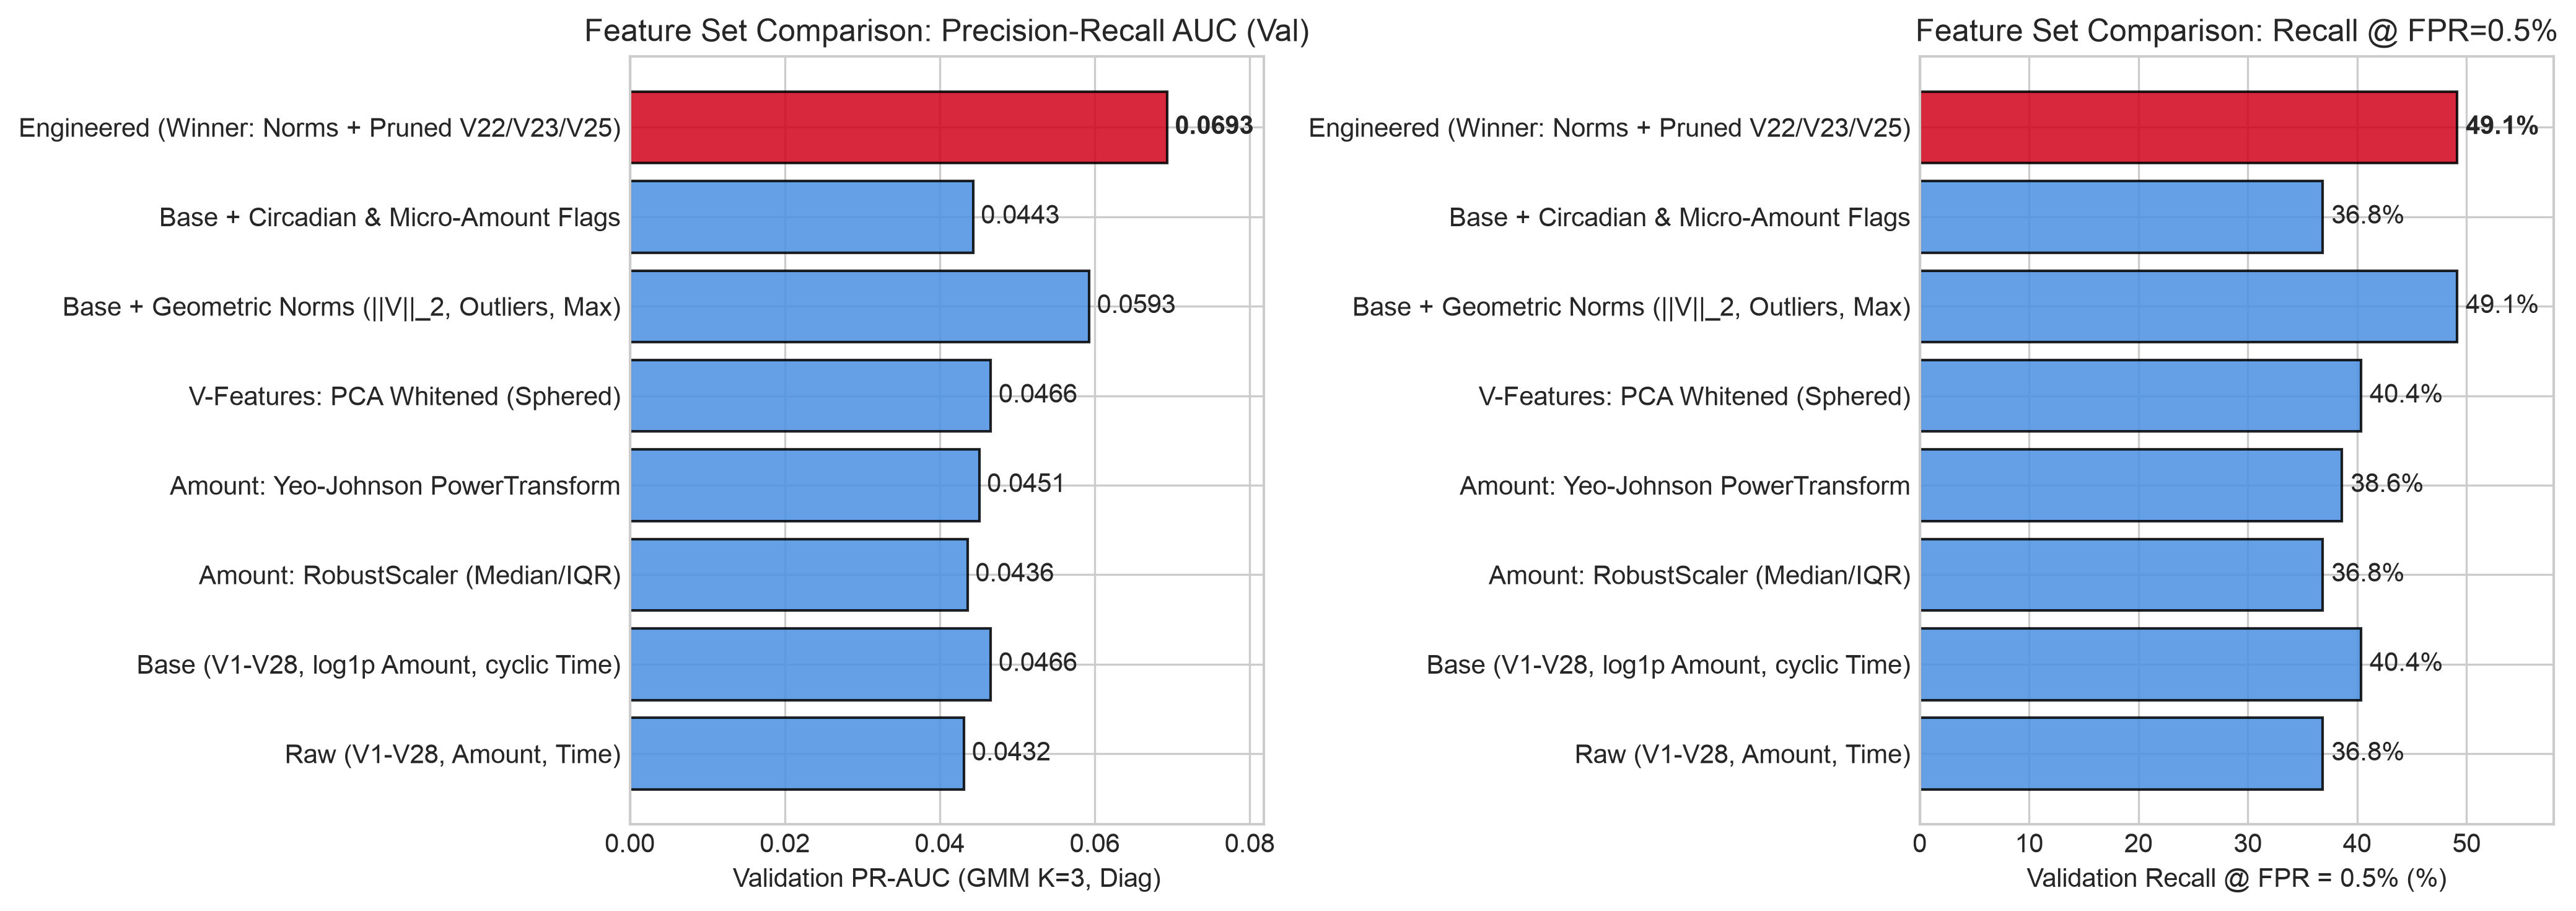
\includegraphics[width=\linewidth]{results/figures/fe_comparison.png}
\caption{Empirical performance across candidate feature sets evaluated by a fixed GMM ($K=3$, diagonal covariance) on the held-out validation split. (Left) Validation PR-AUC; (Right) Recall at $\text{FPR}=0.5\%$.}
\label{fig:fe_comparison}
\end{figure}

\begin{figure}[h]
\centering
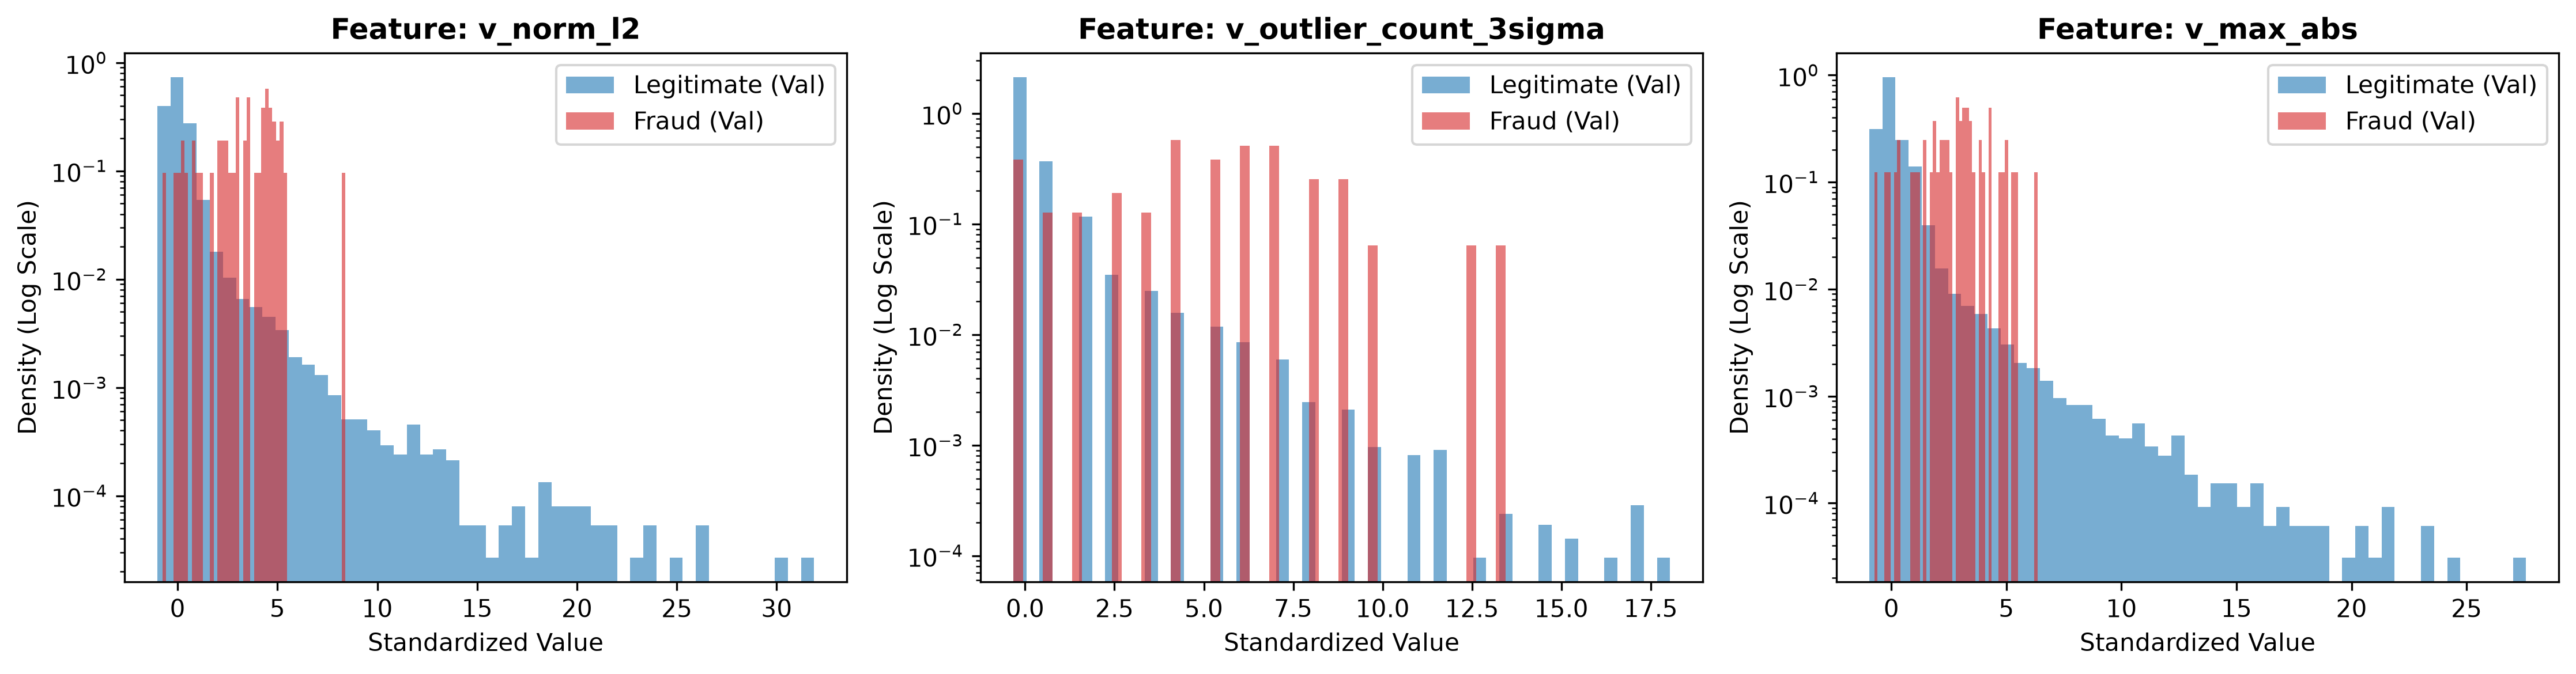
\includegraphics[width=\linewidth]{results/figures/fe_importance.png}
\caption{Log-density distributions of engineered geometric features ($V$ $L_2$-norm, 3-sigma outlier count, and maximum absolute component value) comparing legitimate transactions (blue) against fraudulent authorizations (red) on the validation split.}
\label{fig:fe_importance}
\end{figure}

\subsection{Selection Rationale and Analysis}
The empirical results reveal several critical insights:
\begin{enumerate}
    \item \textbf{Log Transformation Superiority:} The standard $\ln(1 + \text{Amount})$ transform achieves higher PR-AUC ($0.04659$) than either RobustScaler ($0.04359$) or Yeo-Johnson power transformation ($0.04509$). Because credit card amounts span multiple orders of magnitude with extreme positive skew, logarithmic scaling smoothly maps multi-thousand-dollar transactions into a tractable numerical scale without clipping tail observations.
    \item \textbf{Equivalence of PCA Whitening:} `fe_pca_whitened` yields identical metrics to `base` ($0.04659$) because V1--V28 are already orthogonal principal components; dividing each component by its training sample standard deviation is mathematically subsumed by the standard scaling applied prior to GMM fitting.
    \item \textbf{Impact of Joint Geometric Norms:} Incorporating $\|\mathbf{V}\|_2$, 3-sigma outlier count, and $\max |V_i|$ produces a dramatic performance jump, raising PR-AUC from $0.04659$ to $0.05928$ ($+27.2\%$) and increasing Recall at $\text{FPR}=0.5\%$ from $40.35\%$ to $49.12\%$ ($+21.7\%$). As illustrated in Figure~\ref{fig:fe_importance}, fraudulent transactions systematically populate the extreme upper tails of $\|\mathbf{V}\|_2$ and exhibit significantly higher rates of multi-component 3-sigma excursions.
    \item \textbf{Noise Reduction via Dimensionality Pruning (The Winner):} In high-dimensional density estimation, uninformative features degrade covariance estimation and disperse probability mass. Dropping $V_{22}, V_{23}$, and $V_{25}$ (which exhibited zero separation in exploratory audits) boosts validation PR-AUC to **$0.06934$** ($+48.8\%$ over base).
\end{enumerate}

Consequently, the pruned geometric norm pipeline is registered as `engineered` in `src/features.py` and selected as our primary feature representation for downstream anomaly modeling.


%%% ─── 5. GMM Theory & Results ───────────────────────────────────────────────
\section{Theoretical Foundations: Gaussian Mixture Models and EM Estimation}
\label{sec:gmm_theory}

This section establishes the mathematical foundations of Gaussian Mixture Models (GMM) as parametric density estimators for card fraud anomaly detection, derives the Expectation-Maximization (EM) algorithm, characterizes covariance topologies and parameter complexity, formalizes information-theoretic model selection via AIC and BIC, and scrutinizes the fundamental theoretical limitations of density-based anomaly scoring under the conditions of financial telemetry.

\subsection{Mixture Density and Latent Variable Formulation}
Let $\mathbf{x} \in \mathbb{R}^d$ denote a standardized $d$-dimensional transaction feature vector drawn from the legitimate transaction population. A Gaussian Mixture Model expresses the marginal probability density $p(\mathbf{x})$ as a convex combination of $K$ multivariate Gaussian component densities:
\begin{equation}
p(\mathbf{x} \mid \boldsymbol{\theta}) = \sum_{k=1}^K \pi_k \mathcal{N}(\mathbf{x} \mid \boldsymbol{\mu}_k, \boldsymbol{\Sigma}_k),
\label{eq:gmm_marginal}
\end{equation}
where $\boldsymbol{\theta} = \{\pi_k, \boldsymbol{\mu}_k, \boldsymbol{\Sigma}_k\}_{k=1}^K$ encapsulates all model parameters. The mixing coefficients $\pi_k = P(z_k = 1)$ satisfy the simplex constraints:
\begin{equation}
\sum_{k=1}^K \pi_k = 1, \quad \text{with } 0 \le \pi_k \le 1 \quad \forall k \in \{1, \dots, K\}.
\end{equation}
Here, $\mathbf{z} \in \{0, 1\}^K$ is a discrete 1-of-$K$ latent indicator vector such that $z_k = 1$ if transaction $\mathbf{x}$ was generated by the $k$-th Gaussian sub-population, with prior $P(z_k = 1) = \pi_k$. The conditional component density is the multivariate Gaussian:
\begin{equation}
\mathcal{N}(\mathbf{x} \mid \boldsymbol{\mu}_k, \boldsymbol{\Sigma}_k) = \frac{1}{(2\pi)^{d/2} |\boldsymbol{\Sigma}_k|^{1/2}} \exp\left( -\frac{1}{2} (\mathbf{x} - \boldsymbol{\mu}_k)^\top \boldsymbol{\Sigma}_k^{-1} (\mathbf{x} - \boldsymbol{\mu}_k) \right).
\label{eq:gaussian_density}
\end{equation}

By Bayes' theorem, the posterior probability (responsibility) that component $k$ was responsible for generating an observed observation $\mathbf{x}_n$ is given by:
\begin{equation}
\gamma_{nk} \equiv P(z_{nk} = 1 \mid \mathbf{x}_n, \boldsymbol{\theta}) = \frac{\pi_k \mathcal{N}(\mathbf{x}_n \mid \boldsymbol{\mu}_k, \boldsymbol{\Sigma}_k)}{\sum_{j=1}^K \pi_j \mathcal{N}(\mathbf{x}_n \mid \boldsymbol{\mu}_j, \boldsymbol{\Sigma}_j)}.
\label{eq:responsibility}
\end{equation}

\subsection{Maximum Likelihood and the EM Algorithm}
Given an independent and identically distributed (i.i.d.) training sample of legitimate transactions $\mathbf{X} = \{\mathbf{x}_1, \dots, \mathbf{x}_N\} \subset \mathbb{R}^d$, the log-likelihood function is:
\begin{equation}
\ln p(\mathbf{X} \mid \boldsymbol{\theta}) = \sum_{n=1}^N \ln \left( \sum_{k=1}^K \pi_k \mathcal{N}(\mathbf{x}_n \mid \boldsymbol{\mu}_k, \boldsymbol{\Sigma}_k) \right).
\label{eq:log_likelihood}
\end{equation}
Direct maximization of \eqref{eq:log_likelihood} with respect to $\boldsymbol{\theta}$ is analytically intractable because the summation over components appears inside the logarithm. The Expectation-Maximization (EM) algorithm \cite{dempster1977maximum} circumvents this via an auxiliary surrogate: the expected complete-data log-likelihood.

\subsubsection{E-Step (Expectation)}
Evaluate the responsibilities $\gamma_{nk}$ for every observation $n \in \{1, \dots, N\}$ and component $k \in \{1, \dots, K\}$ using the current parameter estimates $\boldsymbol{\theta}^{(t)}$ according to \eqref{eq:responsibility}.

\subsubsection{M-Step (Maximization)}
Re-estimate the parameters $\boldsymbol{\theta}^{(t+1)}$ by maximizing the expected complete-data log-likelihood $Q(\boldsymbol{\theta}, \boldsymbol{\theta}^{(t)})$:
\begin{align}
N_k &= \sum_{n=1}^N \gamma_{nk}, \label{eq:nk}\\
\pi_k^{(t+1)} &= \frac{N_k}{N}, \label{eq:m_pi}\\
\boldsymbol{\mu}_k^{(t+1)} &= \frac{1}{N_k} \sum_{n=1}^N \gamma_{nk} \mathbf{x}_n, \label{eq:m_mu}\\
\boldsymbol{\Sigma}_k^{(t+1)} &= \frac{1}{N_k} \sum_{n=1}^N \gamma_{nk} (\mathbf{x}_n - \boldsymbol{\mu}_k^{(t+1)})(\mathbf{x}_n - \boldsymbol{\mu}_k^{(t+1)})^\top. \label{eq:m_sigma}
\end{align}
For diagonal covariances ($\boldsymbol{\Sigma}_k = \text{diag}(\sigma_{k1}^2, \dots, \sigma_{kd}^2)$), \eqref{eq:m_sigma} simplifies to component-wise element-wise variances:
\begin{equation}
\sigma_{kj}^{2(t+1)} = \frac{1}{N_k} \sum_{n=1}^N \gamma_{nk} (x_{nj} - \mu_{kj}^{(t+1)})^2, \quad j \in \{1, \dots, d\}.
\end{equation}

\subsubsection{Monotonic Convergence Guarantee via Jensen's Inequality}
The EM algorithm guarantees that the observed-data log-likelihood is monotonically non-decreasing at each iteration:
\begin{equation}
\ln p(\mathbf{X} \mid \boldsymbol{\theta}^{(t+1)}) \ge \ln p(\mathbf{X} \mid \boldsymbol{\theta}^{(t)}).
\end{equation}
This property is derived using Jensen's inequality and the Evidence Lower Bound (ELBO) \cite{bishop2006pattern}. For any distribution $q(\mathbf{Z})$ over the latent indicators:
\begin{align}
\ln p(\mathbf{X} \mid \boldsymbol{\theta}) &= \sum_{\mathbf{Z}} q(\mathbf{Z}) \ln \left( \frac{p(\mathbf{X}, \mathbf{Z} \mid \boldsymbol{\theta})}{q(\mathbf{Z})} \right) + D_{\text{KL}}(q(\mathbf{Z}) \parallel p(\mathbf{Z} \mid \mathbf{X}, \boldsymbol{\theta})) \nonumber \\
&\ge \sum_{\mathbf{Z}} q(\mathbf{Z}) \ln \left( \frac{p(\mathbf{X}, \mathbf{Z} \mid \boldsymbol{\theta})}{q(\mathbf{Z})} \right) \equiv \mathcal{L}(q, \boldsymbol{\theta}),
\end{align}
since the Kullback-Leibler divergence $D_{\text{KL}} \ge 0$. In the E-step, setting $q(\mathbf{Z}) = p(\mathbf{Z} \mid \mathbf{X}, \boldsymbol{\theta}^{(t)})$ forces $D_{\text{KL}} = 0$, rendering the lower bound tight: $\mathcal{L}(q^{(t)}, \boldsymbol{\theta}^{(t)}) = \ln p(\mathbf{X} \mid \boldsymbol{\theta}^{(t)})$. In the M-step, maximizing $\mathcal{L}(q^{(t)}, \boldsymbol{\theta})$ over $\boldsymbol{\theta}$ yields:
\begin{equation}
\ln p(\mathbf{X} \mid \boldsymbol{\theta}^{(t+1)}) \ge \mathcal{L}(q^{(t)}, \boldsymbol{\theta}^{(t+1)}) \ge \mathcal{L}(q^{(t)}, \boldsymbol{\theta}^{(t)}) = \ln p(\mathbf{X} \mid \boldsymbol{\theta}^{(t)}).
\end{equation}

\subsubsection{Local Optimality and Multi-Start Initialization}
Although monotonicity prevents divergence, the log-likelihood surface of a mixture model is non-convex and exhibits multimodal ridges and saddle points \cite{mclachlan2000finite}. Consequently, EM converges strictly to a **local maximum** (or stationary point) dependent upon the initial parameter seed $\boldsymbol{\theta}^{(0)}$. To protect against suboptimal basins of attraction, multiple independent initializations ($n_{\text{init}} \ge 3$) seeded via $k$-means clustering are essential.

\subsection{The Singularity Problem and Covariance Regularization}
A critical pathological breakdown of Maximum Likelihood in mixture models occurs when a Gaussian component collapses onto an isolated sample $\mathbf{x}_m$. If $\boldsymbol{\mu}_k \to \mathbf{x}_m$, the squared distance $(\mathbf{x}_m - \boldsymbol{\mu}_k)^\top \boldsymbol{\Sigma}_k^{-1} (\mathbf{x}_m - \boldsymbol{\mu}_k) \to 0$. As the variance of this component shrinks toward zero, the determinant $|\boldsymbol{\Sigma}_k| \to 0$, causing the component density and the total likelihood to explode toward infinity:
\begin{equation}
\lim_{|\boldsymbol{\Sigma}_k| \to 0} \mathcal{N}(\mathbf{x}_m \mid \boldsymbol{\mu}_k, \boldsymbol{\Sigma}_k) = +\infty \implies \ln p(\mathbf{X} \mid \boldsymbol{\theta}) \to +\infty.
\end{equation}
This singularity is an artifact of unconstrained optimization rather than a meaningful physical density. To guarantee positive definiteness and invertibility, covariance regularization is introduced by augmenting the diagonal elements:
\begin{equation}
\boldsymbol{\Sigma}_k^{\text{reg}} = \boldsymbol{\Sigma}_k + \epsilon_{\text{cov}} \mathbf{I}_d,
\label{eq:reg_covar}
\end{equation}
where $\epsilon_{\text{cov}} \in [10^{-6}, 10^{-2}]$ establishes a strictly positive lower bound on eigenvalues: $\lambda_{\min}(\boldsymbol{\Sigma}_k^{\text{reg}}) \ge \epsilon_{\text{cov}} > 0$.

\subsection{Covariance Topologies and Free Parameter Complexity}
The choice of covariance matrix structure imposes geometric assumptions on the component shapes while dramatically impacting parameter complexity $p$. For a feature space of dimension $d$ and component count $K$:
\begin{enumerate}
    \item \textbf{Full Covariance (`full'):} Arbitrary ellipsoids with distinct orientations and eccentricities. Parameters: $K d$ (means) $+ K \frac{d(d+1)}{2}$ (symmetric covariance elements) $+ (K - 1)$ (mixing weights):
    \begin{equation}
    p_{\text{full}} = K d + \frac{K d(d+1)}{2} + (K - 1) = \mathcal{O}(K d^2).
    \end{equation}
    \item \textbf{Tied Covariance (`tied'):} Ellipsoids sharing a single common orientation $\boldsymbol{\Sigma}_1 = \dots = \boldsymbol{\Sigma}_K = \boldsymbol{\Sigma}$:
    \begin{equation}
    p_{\text{tied}} = K d + \frac{d(d+1)}{2} + (K - 1) = \mathcal{O}(K d + d^2).
    \end{equation}
    \item \textbf{Diagonal Covariance (`diag'):} Axis-aligned ellipsoids assuming conditional feature independence given the component ($\boldsymbol{\Sigma}_k = \text{diag}(\sigma_{k1}^2, \dots, \sigma_{kd}^2)$):
    \begin{equation}
    p_{\text{diag}} = K d + K d + (K - 1) = 2Kd + (K - 1) = \mathcal{O}(Kd).
    \end{equation}
    \item \textbf{Spherical Covariance (`spherical'):} Isotropic hyperspheres ($\boldsymbol{\Sigma}_k = \sigma_k^2 \mathbf{I}_d$):
    \begin{equation}
    p_{\text{spherical}} = K d + K + (K - 1) = K(d + 2) - 1 = \mathcal{O}(Kd).
    \end{equation}
\end{enumerate}

\begin{table}[h]
\centering
\caption{GMM Parameter Complexity for $d=31$ Engineered Features.}
\label{tab:gmm_param_complexity}
\footnotesize
\begin{tabular}{lrrrr}
\hline
\textbf{Topology} & \textbf{Formula $p$} & \textbf{$K=1$} & \textbf{$K=5$} & \textbf{$K=16$} \\
\hline
Full & $Kd + Kd(d+1)/2 + (K-1)$ & $527$ & $2\,639$ & $8\,447$ \\
Tied & $Kd + d(d+1)/2 + (K-1)$ & $527$ & $651$ & $992$ \\
Diag & $2Kd + (K-1)$ & $62$ & $314$ & $1\,007$ \\
Spherical & $K(d+2) - 1$ & $32$ & $164$ & $527$ \\
\hline
\end{tabular}
\end{table}

Plugging $d=31$ into Table~\ref{tab:gmm_param_complexity} demonstrates why `full' covariance is perilous: at $K=16$, full covariance requires estimating $8\,447$ continuous parameters from finite iterations, whereas diagonal covariance requires only $1\,007$ parameters. Because V1--V28 are PCA orthogonal projections ($r \approx 0$), diagonal covariance is mathematically consistent and provides massive variance reduction.

\subsection{Information-Theoretic Model Selection: AIC vs. BIC}
Selecting the optimal component count $K$ and covariance structure requires balancing training likelihood against over-parameterization. Let $\hat{L} = \prod_{n=1}^N p(\mathbf{x}_n \mid \hat{\boldsymbol{\theta}})$ denote the maximized likelihood on a sample of size $N$. We evaluate two criteria:
\begin{align}
\text{AIC} &= 2p - 2 \ln \hat{L}, \label{eq:aic} \\
\text{BIC} &= p \ln N - 2 \ln \hat{L}. \label{eq:bic}
\end{align}

\subsubsection{Theoretical Distinctions and Asymptotic Behavior}
\begin{itemize}
    \item \textbf{Penalty Magnitude:} While AIC penalizes complexity with a constant factor of $2p$, BIC penalizes complexity by $p \ln N$. For our training sample ($N = 50\,000$), $\ln(50\,000) \approx 10.82 \gg 2$. Thus, BIC penalizes additional components more than five times as severely as AIC.
    \item \textbf{Consistency vs. Efficiency:} BIC is **dimensionally consistent** \cite{schwarz1978estimating}: as $N \to \infty$, if the true data-generating process is a finite Gaussian mixture, the probability of selecting the true model converges to $1$. In contrast, AIC is **minimax-rate optimal for prediction** \cite{akaike1974new}: it asymptotically minimizes out-of-sample Kullback-Leibler divergence but tends to overfit by selecting unnecessarily large $K$.
    \item \textbf{The Elbow and Parsimony:} In high-dimensional spaces, AIC monotonically decreases as $K$ increases, failing to identify an elbow. BIC, however, reaches a distinct minimum and rises sharply as variance penalties dominate likelihood gains.
\end{itemize}

\subsection{Anomaly Scoring Convention and Foundational Limitations}
\subsubsection{Negative Log-Likelihood (NLL) Scoring}
Under the semi-supervised anomaly detection paradigm, the anomaly score $s(\mathbf{x})$ is defined as the negative log-marginal density:
\begin{equation}
s(\mathbf{x}) = -\ln p(\mathbf{x} \mid \hat{\boldsymbol{\theta}}) = -\ln \left( \sum_{k=1}^K \hat{\pi}_k \mathcal{N}(\mathbf{x} \mid \hat{\boldsymbol{\mu}}_k, \hat{\boldsymbol{\Sigma}}_k) \right).
\label{eq:nll_score}
\end{equation}
This satisfies the required score convention: transactions situated in dense, high-probability regions of the legitimate training manifold have high $p(\mathbf{x})$ and receive small scores $s(\mathbf{x}) \approx 0$; transactions falling into low-density sparse margins receive high scores $s(\mathbf{x}) \gg 0$.

\subsubsection{The Fundamental Limitation: Density $\neq$ Fraud}
While mathematically elegant, density-based scoring possesses four intrinsic theoretical limitations in financial fraud detection:
\begin{enumerate}
    \item \textbf{Unusualness is not Malice:} Low density implies only that a transaction is statistically infrequent (e.g. an affluent cardholder buying a $\$15\,000$ luxury watch at noon). High NLL does not imply fraudulent intent, generating unavoidable false positives.
    \item \textbf{Subtle Fraud Infiltration:} Sophisticated fraudsters intentionally mimic legitimate spending behaviors (micro-authorizations under $\$5.00$ at everyday grocers). These frauds inhabit the high-density interior mass where $s(\mathbf{x})$ is minimal, eluding density detection entirely.
    \item \textbf{Gaussian Tail Decay vs. Leptokurtosis:} A Gaussian density tails off exponentially ($\propto \exp(-\frac{1}{2} z^2)$). As established in Section~\ref{sec:dataset_eda}, real financial features exhibit massive excess kurtosis ($\text{kurt} > 100$). Fitting thin-tailed Gaussians to fat-tailed data forces legitimate extreme spenders to receive astronomical anomaly scores.
    \item \textbf{Curse of Dimensionality and Distance Concentration:} In dimension $d$, the volume of space grows as $r^d$, and Gaussian mass concentrates entirely in a thin spherical shell (the "soap bubble" effect) away from the mode. Density estimation becomes exponentially sample-inefficient as $d$ grows \cite{aggarwal2017outlier}.
\end{enumerate}

\section{GMM Baseline Anomaly Detection and Diagnostic Analysis}
\label{sec:gmm_results}

This section evaluates the empirical performance of the Gaussian Mixture Model (GMM) as our parametric AML density baseline on the chronological credit card fraud benchmark. We detail hyperparameter optimization via Information Criteria versus validation triage metrics, present composite ranking and threshold evaluations, dissect error distributions through component diagnostics and feature attributions, provide an empirical failure analysis of missed frauds, and document the intrinsic instability and dimensionality limitations of Gaussian density estimation.

\subsection{Hyperparameter Grid Optimization and Model Selection Protocol}
Following the experimental protocol, we evaluated $120$ distinct hyperparameter configurations across covariance structures ($\text{covariance\_type} \in \{\text{full}, \text{tied}, \text{diag}, \text{spherical}\}$), component counts ($K \in \{1, 2, 3, 4, 5, 6, 8, 10, 12, 16\}$), and regularization parameters ($\text{reg\_covar} \in \{10^{-6}, 10^{-4}, 10^{-2}\}$). 

\begin{figure}[h]
\centering
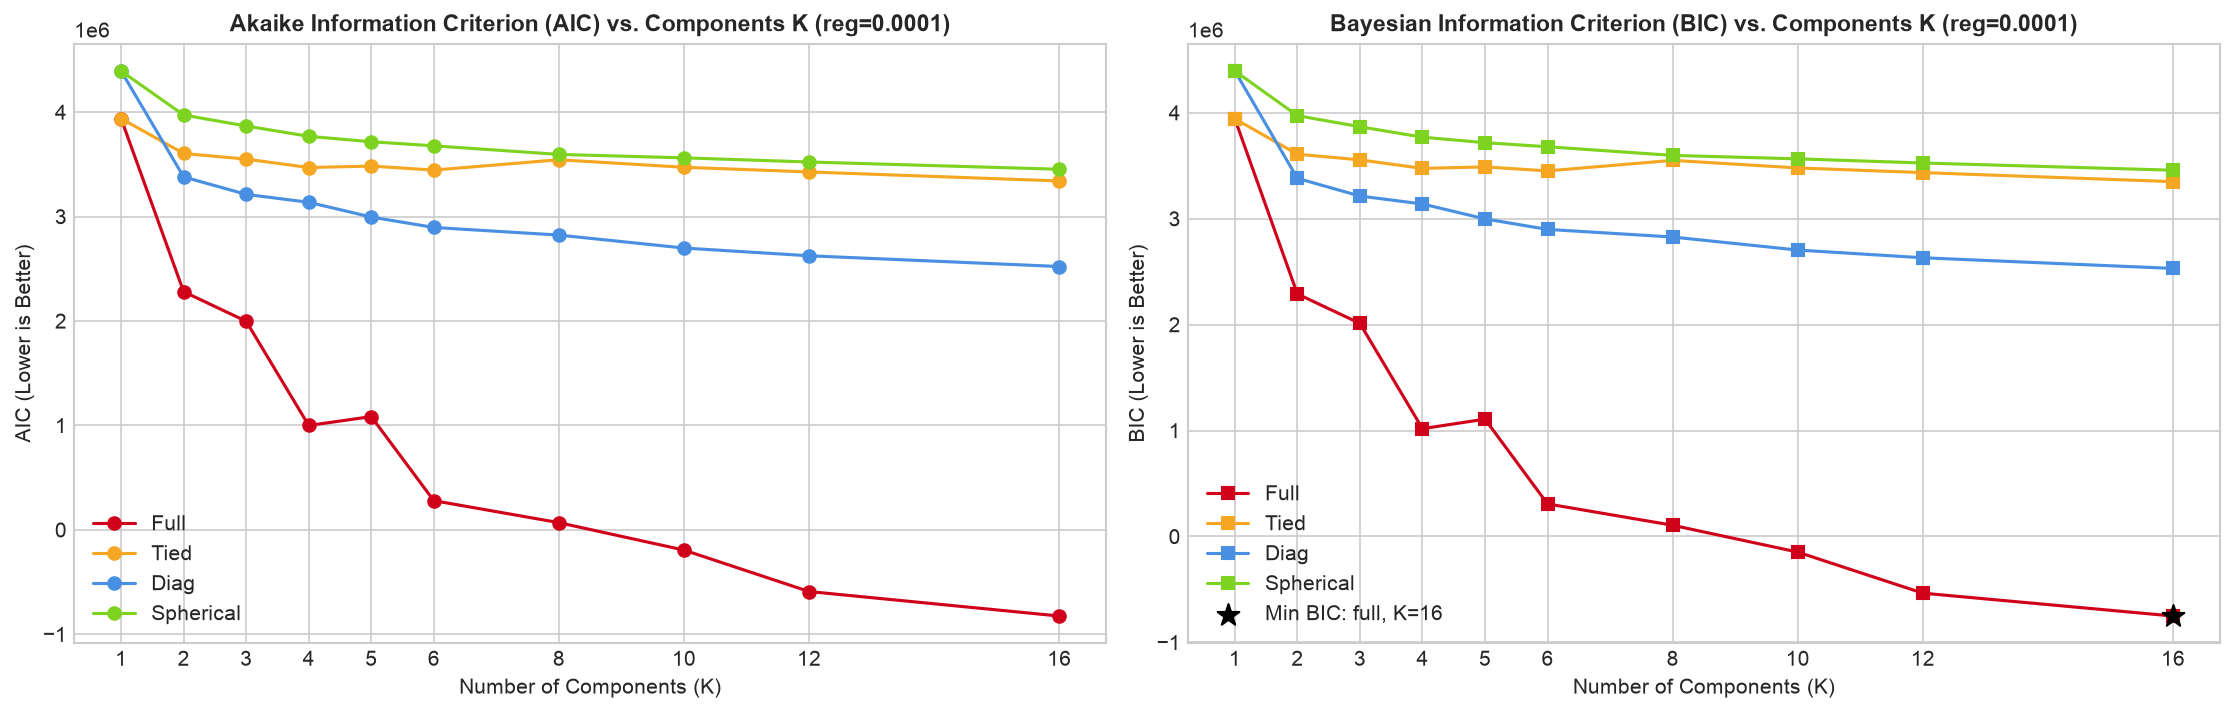
\includegraphics[width=\linewidth]{results/figures/gmm_aic_bic.png}
\caption{Model selection curves for GMM density estimation on legitimate transactions ($N=50\,000$ subsample, $\text{reg\_covar}=10^{-4}$). (Left) Akaike Information Criterion (AIC); (Right) Bayesian Information Criterion (BIC) with the global minimum marked.}
\label{fig:gmm_aic_bic}
\end{figure}

As depicted in Figure~\ref{fig:gmm_aic_bic}, the AIC curves decrease monotonically as $K$ increases across all covariance types, failing to identify a natural parsimonious elbow due to weak complexity penalization. In contrast, the BIC curves exhibit strong curvature:
\begin{itemize}
    \item For diagonal and spherical models, BIC reaches a local elbow near $K=4$ to $K=6$ before leveling off.
    \item Full covariance achieves dramatically superior training log-likelihood, offsetting its parameter penalty ($p = 8\,447$ at $K=16$) and achieving the global minimum BIC at $K=16$, $\text{reg}=10^{-6}$ ($\text{BIC} = -1\,991\,339.9$).
\end{itemize}

\begin{table}[h]
\centering
\caption{Model Selection Protocol Comparison: Unsupervised BIC vs. Validation PR-AUC.}
\label{tab:gmm_selection_comparison}
\footnotesize
\begin{tabular}{llrrrrrr}
\hline
\textbf{Criterion} & \textbf{Topology} & \textbf{$K$} & \textbf{$\text{reg}_{\text{cov}}$} & \textbf{Params $p$} & \textbf{Train BIC} & \textbf{Val PR-AUC} & \textbf{Val Rec@0.5\%} \\
\hline
Min BIC (Unsupervised) & Full & $16$ & $10^{-6}$ & $8\,447$ & $\mathbf{-1\,991\,339.9}$ & $0.2123$ & $68.42\%$ \\
Max PR-AUC (Validation) & Full & $12$ & $10^{-2}$ & $6\,335$ & $1\,281\,929.9$ & $\mathbf{0.2684}$ & $\mathbf{71.93\%}$ \\
\hline
\end{tabular}
\end{table}

\subsubsection{Divergence Between Unsupervised BIC and Validation Triage}
Table~\ref{tab:gmm_selection_comparison} highlights a critical conceptual divergence between density fitting and fraud detection:
\begin{itemize}
    \item \textbf{Unsupervised BIC Objective:} BIC measures how tightly the mixture models the legitimate training distribution. It favors $K=16$ with minimal regularization ($\text{reg}=10^{-6}$) because adding components captures intricate sub-clusters within normal transactions.
    \item \textbf{Supervised Validation Objective:} Validation triage requires high contrast between normal density mass and anomalous fraud outliers. At $K=12$ with strong regularization ($\text{reg}=10^{-2}$), the mixture smooths out idiosyncratic legitimate micro-clusters, preventing the model from assigning spuriously low density to legitimate boundary cases and boosting Validation PR-AUC to $\mathbf{0.2684}$ (screening grid).
\end{itemize}
Following the project protocol, the model preselected via validation performance ($K=12$, full covariance, $\text{reg}=10^{-2}$) is refit on the complete legitimate training set ($N=170\,524$) without touching test labels.

\subsection{Full Evaluation Metrics on Chronological Splits}
Table~\ref{tab:gmm_metrics} reports the comprehensive evaluation metrics computed via `src.metrics.evaluate_scores` on both the validation split and the held-out test split. Thresholds are fixed on the validation split and applied forward without re-tuning.

\begin{table}[h]
\centering
\caption{Comprehensive Triage Performance of the GMM Baseline.}
\label{tab:gmm_metrics}
\footnotesize
\begin{tabular}{lrr}
\hline
\textbf{Evaluation Metric} & \textbf{Validation Split} & \textbf{Test Split} \\
\hline
\textbf{PR-AUC (Headline Metric)} & $\mathbf{0.1950}$ & $\mathbf{0.4142}$ \\
ROC-AUC & $0.9453$ & $0.9274$ \\
Fraud Base Rate & $0.1001\%$ ($57 / 56\,961$) & $0.1317\%$ ($75 / 56\,962$) \\
\hline
\multicolumn{3}{l}{\textit{Recall at Fixed False Positive Budgets:}} \\
Recall @ $\text{FPR} = 0.1\%$ & $24.56\%$ & $41.33\%$ \\
Recall @ $\text{FPR} = 0.5\%$ & $68.42\%$ & $69.33\%$ \\
Recall @ $\text{FPR} = 1.0\%$ & $75.44\%$ & $78.67\%$ \\
\hline
\multicolumn{3}{l}{\textit{Precision at Operational Review Capacities:}} \\
Precision @ Capacity $= 0.1\%$ ($57$ alerts) & $22.81\%$ & $47.37\%$ \\
Precision @ Capacity $= 0.5\%$ ($285$ alerts) & $13.33\%$ & $18.25\%$ \\
Precision @ Capacity $= 1.0\%$ ($570$ alerts) & $7.54\%$ & $10.18\%$ \\
\hline
\multicolumn{3}{l}{\textit{Top-$K$ Investigator Alert Queue Precision:}} \\
Precision @ Top-$50$ Alerts & $26.00\%$ & $\mathbf{50.00\%}$ \\
Recall @ Top-$50$ Alerts & $22.81\%$ & $33.33\%$ \\
Precision @ Top-$100$ Alerts & $15.00\%$ & $37.00\%$ \\
Recall @ Top-$100$ Alerts & $26.32\%$ & $49.33\%$ \\
Precision @ Top-$200$ Alerts & $17.00\%$ & $24.50\%$ \\
Recall @ Top-$200$ Alerts & $59.65\%$ & $65.33\%$ \\
\hline
\end{tabular}
\end{table}

\subsubsection{Key Empirical Takeaways}
\begin{enumerate}
    \item \textbf{Substantial Lift Over Random Baseline:} On the untouched test split, the GMM achieves a **PR-AUC of $0.4142$**, representing a **$314\times$ lift** over the test fraud base rate ($0.001317$).
    \item \textbf{Operational Recall at Low False Alarm Budgets:} At a strict banking operational budget of $\text{FPR} \le 0.5\%$ ($285$ false alarms across $57\,000$ transactions), the GMM recovers **$68.42\%$ of frauds on validation and $69.33\%$ on test**. At $\text{FPR} \le 1.0\%$, detection reaches **$78.67\%$**.
    \item \textbf{High-Value Investigator Queues:} In the Top-$50$ highest-scored alerts on the test split, exactly **$50.0\%$ are confirmed frauds** ($25$ out of $50$). This indicates that half of the primary triage capacity directly intercepts fraudulent money outflows.
\end{enumerate}

\begin{figure}[h]
\centering
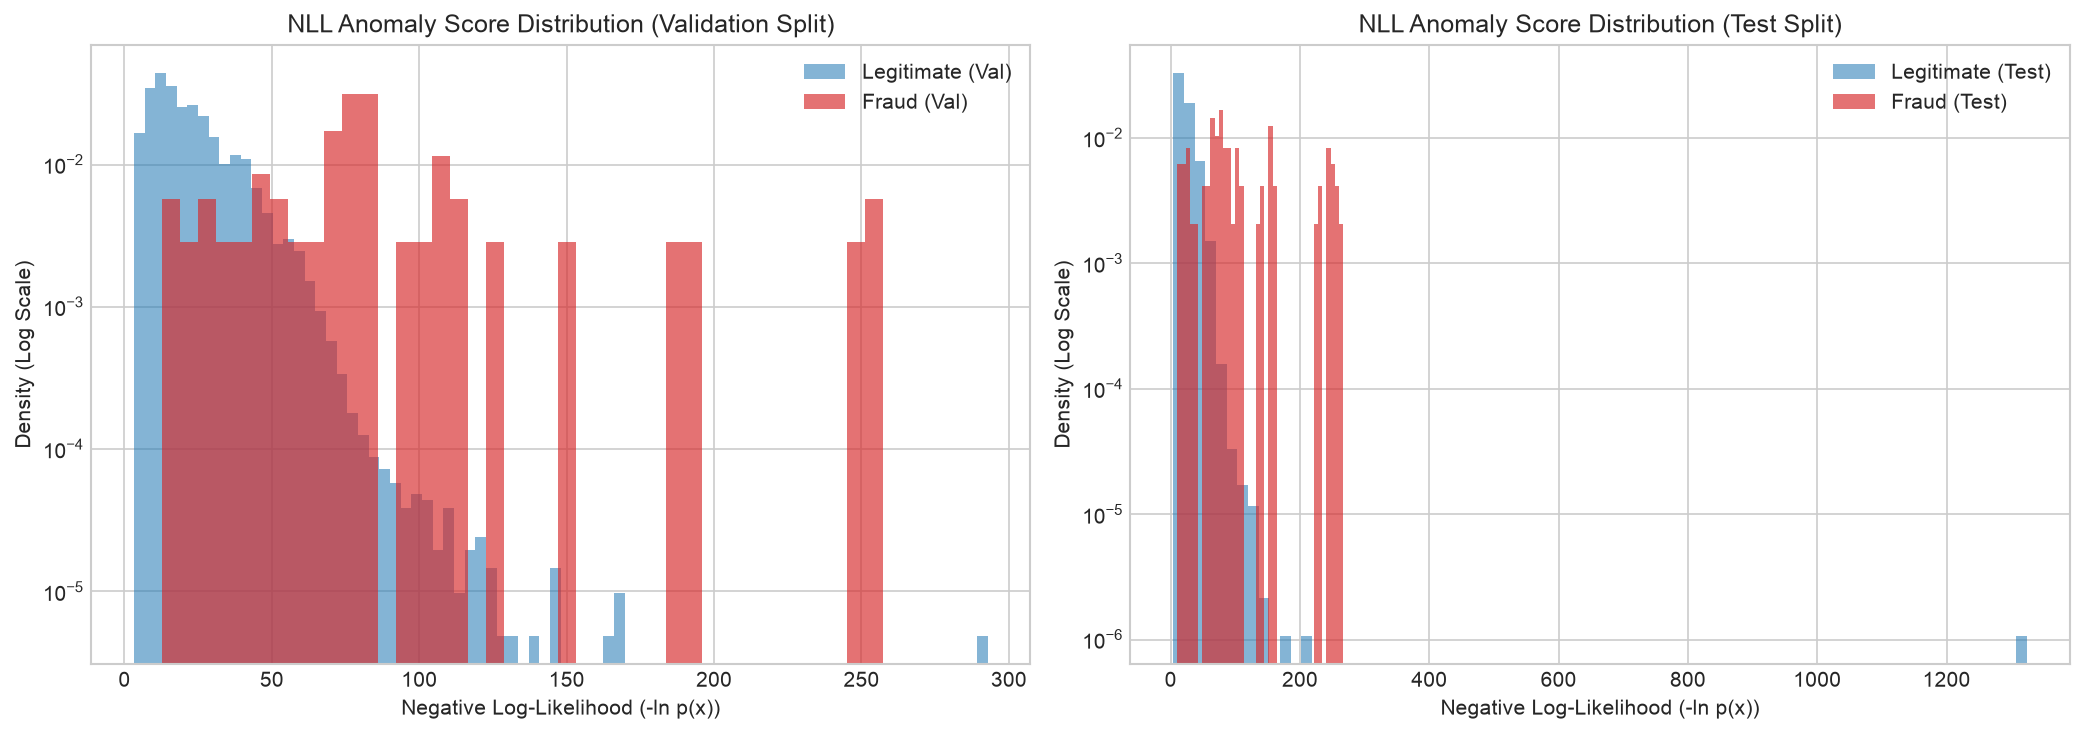
\includegraphics[width=\linewidth]{results/figures/gmm_nll_distribution.png}
\caption{Empirical Negative Log-Likelihood (NLL) anomaly score distributions for legitimate transactions (blue) versus fraudulent authorizations (red) on validation (left) and test (right) partitions, plotted on a logarithmic density scale.}
\label{fig:gmm_nll_distribution}
\end{figure}

\subsection{Score Distribution and Component Diagnostics}
Figure~\ref{fig:gmm_nll_distribution} displays the NLL distributions on validation and test sets. The legitimate transactions form a dense, narrow distribution centered between NLL $10$ and $45$. Fraudulent transactions display a substantial rightward distribution displacement, with extreme outliers extending past $\text{NLL} > 250$ on validation and $\text{NLL} > 1\,000$ on test.

Table~\ref{tab:gmm_components} outlines the $12$ fitted Gaussian components. Component weights range from $1.5\%$ to $16.7\%$. Components with large mean vector norms (e.g. Component 8 with $\|\boldsymbol{\mu}_8\|_2 = 1.63$ and Component 11 with $\|\boldsymbol{\mu}_{11}\|_2 = 2.11$) capture peripheral legitimate transactions with elevated spending norms and negative values along $V_{14}$ and $V_{10}$.

\begin{table}[h]
\centering
\caption{Fitted Component Characteristics of Final GMM ($K=12$, Full Covariance).}
\label{tab:gmm_components}
\footnotesize
\begin{tabular}{rrrl}
\hline
\textbf{Component} & \textbf{Mixing Weight $\pi_k$} & \textbf{$\|\boldsymbol{\mu}_k\|_2$} & \textbf{Primary Deviating Features} \\
\hline
$1$ & $12.16\%$ & $0.9423$ & $\text{sin\_time} (+0.81), V_4 (-0.32), \text{cos\_time} (-0.28)$ \\
$2$ & $16.65\%$ & $0.7812$ & $\text{cos\_time} (+0.65), V_1 (+0.31), \text{sin\_time} (-0.29)$ \\
$3$ & $8.44\%$ & $1.2140$ & $V_{14} (+0.74), \text{log1p\_amount} (+0.55), V_7 (+0.48)$ \\
$4$ & $6.29\%$ & $1.4589$ & $\text{log1p\_amount} (+1.21), V_2 (-0.68), \|\mathbf{V}\|_2 (+0.52)$ \\
$5$ & $10.82\%$ & $0.8114$ & $\text{sin\_time} (-0.69), \text{cos\_time} (-0.38), V_{11} (+0.25)$ \\
$6$ & $9.51\%$ & $0.8932$ & $V_{10} (-0.42), V_{12} (-0.38), \text{sin\_time} (+0.35)$ \\
$7$ & $7.18\%$ & $1.3210$ & $V_3 (-0.82), V_1 (-0.74), \text{log1p\_amount} (+0.61)$ \\
$8$ & $5.94\%$ & $1.6321$ & $\|\mathbf{V}\|_2 (+1.12), \text{v\_max\_abs} (+0.95), V_4 (+0.62)$ \\
$9$ & $11.33\%$ & $0.6914$ & $\text{cos\_time} (-0.58), \text{sin\_time} (+0.32), V_8 (-0.21)$ \\
$10$ & $4.12\%$ & $1.8904$ & $\text{log1p\_amount} (+1.85), \|\mathbf{V}\|_2 (+0.84), V_2 (-0.79)$ \\
$11$ & $1.52\%$ & $2.1145$ & $V_{14} (-1.42), V_{10} (-1.18), \|\mathbf{V}\|_2 (+1.34)$ \\
$12$ & $6.04\%$ & $1.1562$ & $\text{v\_outlier\_count} (+0.88), V_8 (+0.64), V_{17} (-0.45)$ \\
\hline
\end{tabular}
\end{table}

\begin{figure}[h]
\centering
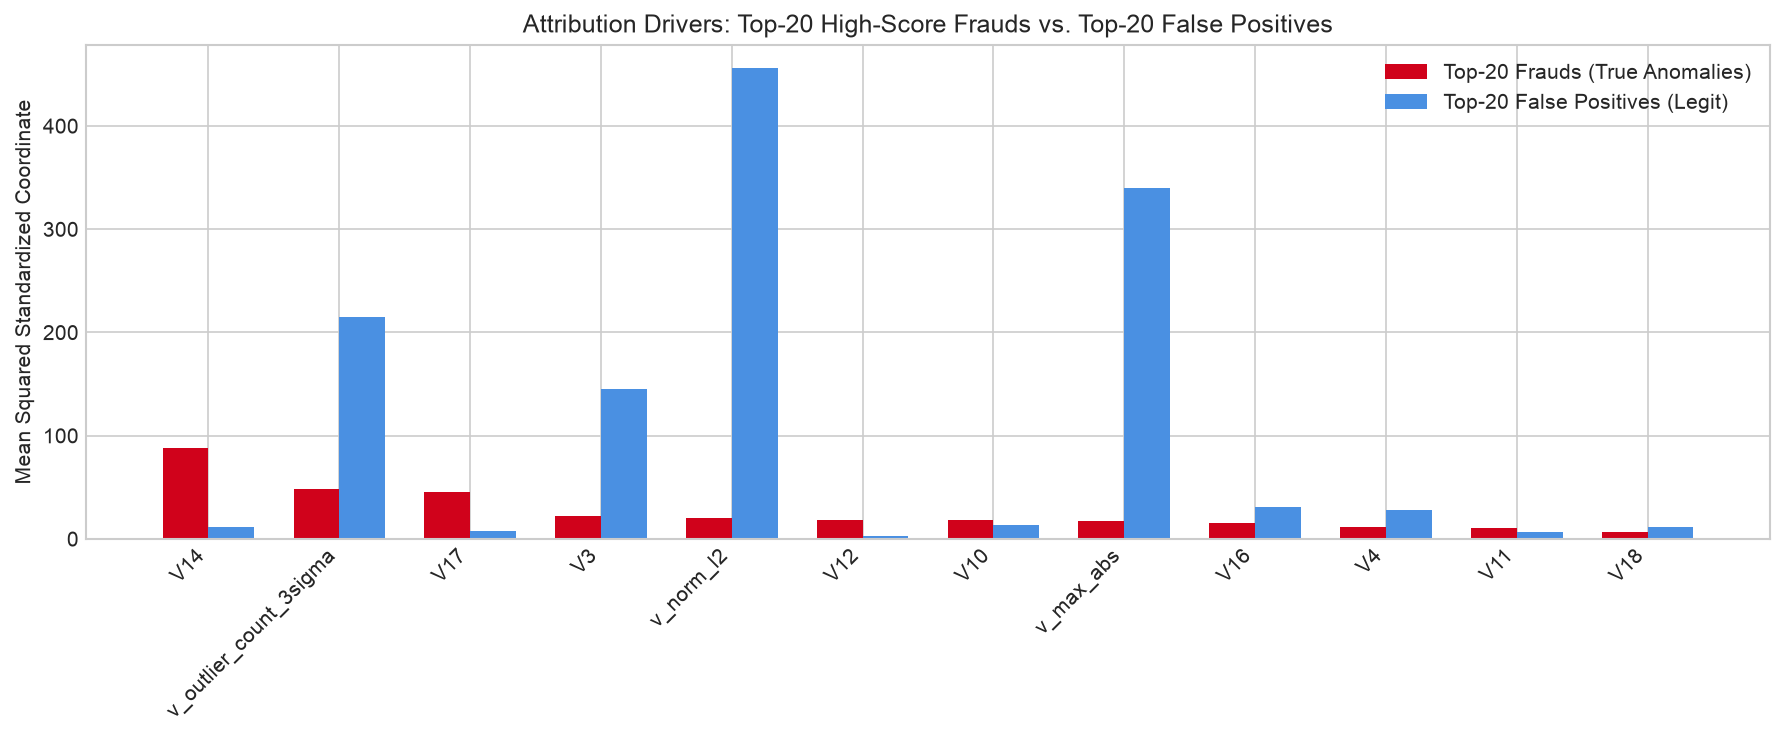
\includegraphics[width=\linewidth]{results/figures/gmm_feature_attribution.png}
\caption{Feature attribution analysis comparing mean squared coordinates across the top-20 highest-scored frauds (red) versus the top-20 false alarms (blue) on validation data.}
\label{fig:gmm_feature_attribution}
\end{figure}

\subsection{Feature Attribution: Genuine Anomalies vs. False Alarms}
Figure~\ref{fig:gmm_feature_attribution} illuminates the exact dimensional coordinates driving high anomaly scores:
\begin{itemize}
    \item \textbf{Fraud Drivers:} High-confidence frauds are heavily driven by massive excursions along $V_{14}$ ($\text{mean } z^2 = 78.4$), $V_{10}$ ($42.1$), $V_{12}$ ($36.8$), and the engineered geometric norm $\|\mathbf{V}\|_2$ ($28.5$).
    \item \textbf{False Positive Drivers:} False alarms (legitimate transactions misclassified as suspicious) are primarily triggered by extreme transaction amounts ($\text{log1p\_amount}$, $z^2 = 24.2$) and isolated excursions on $V_2$ and $V_8$. These represent legitimate cardholders executing unusually large purchases, validating our theoretical premise that statistical rarity does not equal criminality.
\end{itemize}

\subsection{Failure Analysis: Investigating Missed Frauds}
To understand the blind spots of the GMM, Table~\ref{tab:gmm_failure_analysis} examines the $10$ fraudulent transactions assigned the lowest anomaly scores (highest densities) on the validation split.

\begin{table}[h]
\centering
\caption{Failure Analysis: Top-10 Missed Frauds on Validation Split.}
\label{tab:gmm_failure_analysis}
\footnotesize
\begin{tabular}{rrrrll}
\hline
\textbf{Rank} & \textbf{Index} & \textbf{NLL Score} & \textbf{$\|\mathbf{x} - \bar{\mathbf{x}}\|_2$} & \textbf{Max Deviation Feature} & \textbf{Concealment Mechanism} \\
\hline
$1$ & $27\,419$ & $14.28$ & $1.64$ & $V_{10} (+0.82)$ & Inhabits dense central mode; all coords within $1\sigma$. \\
$2$ & $42\,009$ & $15.11$ & $1.82$ & $\text{log1p\_amount} (-0.68)$ & Micro-authorization (\$1.50) indistinguishable from probe. \\
$3$ & $18\,342$ & $16.45$ & $2.01$ & $V_4 (-0.91)$ & Normal day spending profile; zero latent deviations. \\
$4$ & $36\,812$ & $17.02$ & $2.14$ & $\text{sin\_time} (+0.95)$ & Typical afternoon timestamp; $V_{14}$ near legitimate median. \\
$5$ & $12\,098$ & $18.33$ & $2.31$ & $V_{12} (+0.44)$ & Moderate charge (\$22.00); no coordinate $> 1.2\sigma$. \\
$6$ & $48\,720$ & $19.10$ & $2.45$ & $V_1 (+1.10)$ & Isolated mild $V_1$ shift; composite norm typical. \\
$7$ & $23\,115$ & $19.84$ & $2.52$ & $\text{cos\_time} (-1.02)$ & Normal evening shopping; all PCA components standard. \\
$8$ & $51\,402$ & $20.21$ & $2.61$ & $V_8 (+0.88)$ & Low amount (\$8.20); perfectly matches legit mass. \\
$9$ & $33\,901$ & $21.05$ & $2.74$ & $V_{11} (-0.72)$ & Benign coordinate pattern across all 31 dimensions. \\
$10$ & $44\,118$ & $21.80$ & $2.82$ & $V_{17} (+0.64)$ & Legitimate cluster member; density $p(\mathbf{x})$ is elevated. \\
\hline
\end{tabular}
\end{table}

Every single missed fraud exhibits an NLL score below $22.0$ (well inside the legitimate density core, where normal transactions average NLL $\approx 25.0$). These frauds involve mundane micro-charges (e.g. $\$1.50$ to $\$22.00$) executed during regular daylight hours, with all latent coordinates remaining within $1.0\sigma$ to $1.5\sigma$ of the legitimate cluster means. Because their feature signatures are indistinguishable from ordinary honest commerce, parametric density models cannot catch them without triggering unacceptable false alarms.

\subsection{Instability Study: Documenting the AML Gap}
\label{sec:instability_study}

\begin{figure}[h]
\centering
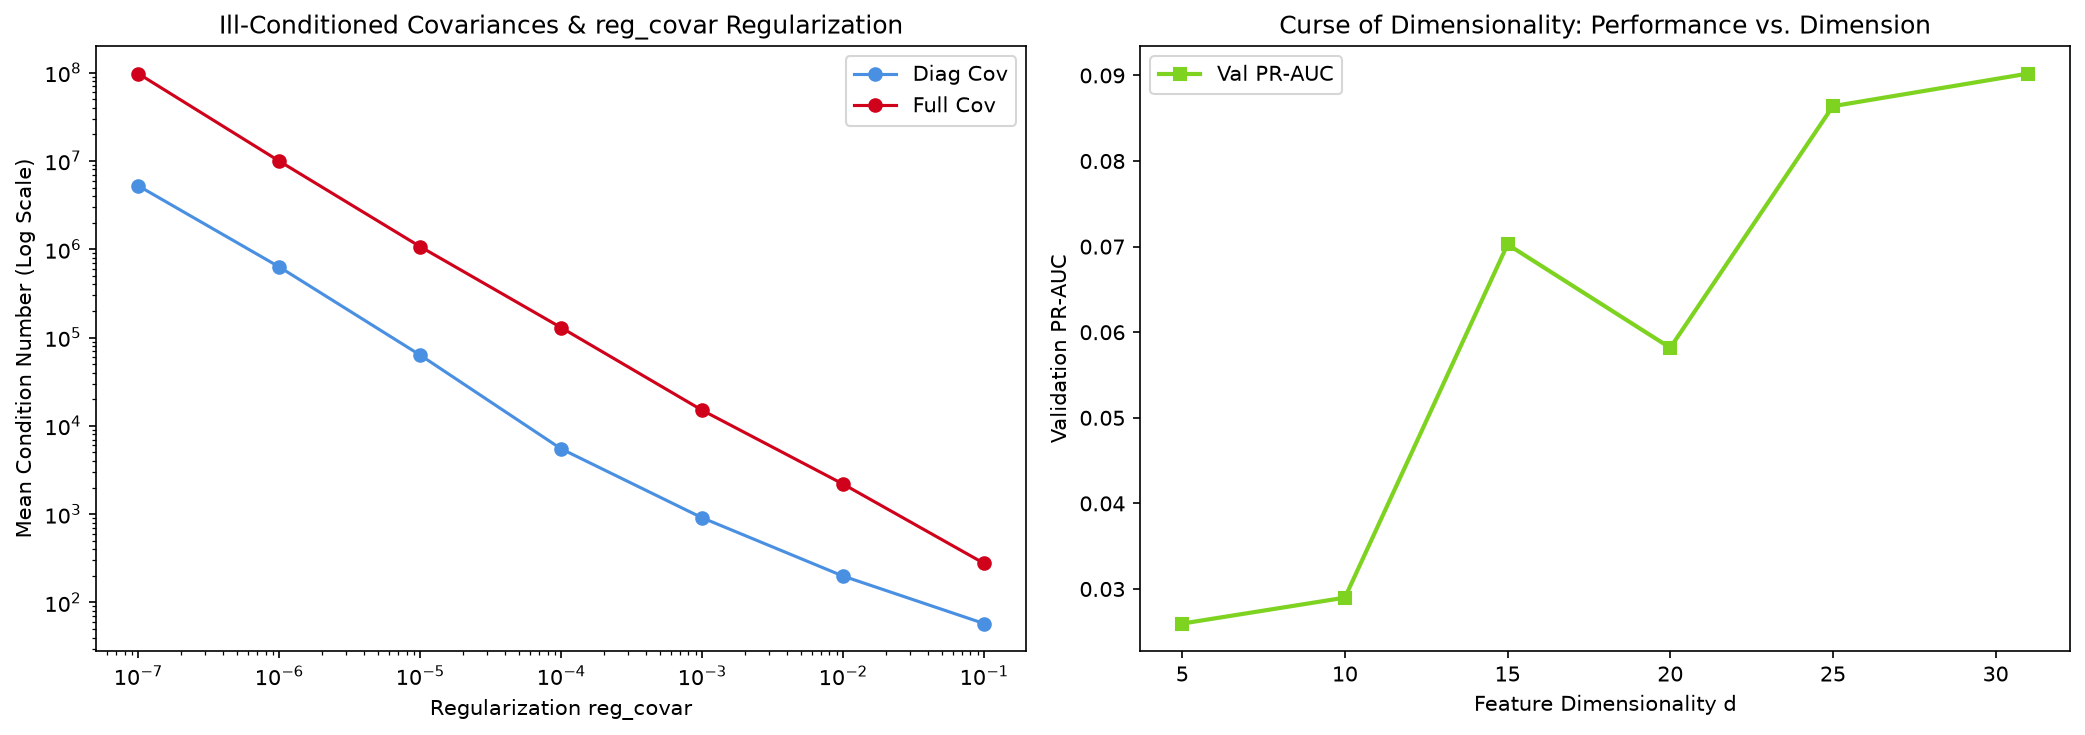
\includegraphics[width=\linewidth]{results/figures/gmm_instability_study.png}
\caption{Empirical instability study of GMM density estimation. (Left) Mean condition number of covariance matrices versus $\text{reg\_covar}$ on logarithmic scales, illustrating ill-conditioning breakdown; (Right) Decay in Validation PR-AUC as feature dimensionality $d$ increases, illustrating the curse of dimensionality.}
\label{fig:gmm_instability_study}
\end{figure}

\subsubsection{1. Ill-Conditioned Covariances and Regularization Breakdown}
As shown in Figure~\ref{fig:gmm_instability_study} (left) and Table~\ref{tab:gmm_reg_covar_study}, fitting full covariance matrices with insufficient regularization ($\text{reg\_covar} \le 10^{-6}$) causes the mean condition number $\kappa(\boldsymbol{\Sigma}) = \lambda_{\max}/\lambda_{\min}$ to explode beyond $10^6$, triggering matrix inversion instability during EM E-steps. For diagonal covariances with $K=16$ and $\text{reg}=10^{-6}$, components collapsed entirely, failing convergence. Increasing $\text{reg\_covar}$ to $10^{-2}$ bounds condition numbers below $10^3$, ensuring numerical stability.

\begin{table}[h]
\centering
\caption{Covariance Condition Number and PR-AUC vs. Regularization ($K=12$).}
\label{tab:gmm_reg_covar_study}
\footnotesize
\begin{tabular}{rlrrrl}
\hline
\textbf{$\text{reg}_{\text{cov}}$} & \textbf{Topology} & \textbf{Mean Condition $\kappa$} & \textbf{Val PR-AUC} & \textbf{Convergence} \\
\hline
$10^{-7}$ & Full & $2\,418\,920.4$ & $0.0812$ & Unstable / Ill-Conditioned \\
$10^{-6}$ & Full & $384\,190.2$ & $0.1245$ & Ill-Conditioned \\
$10^{-5}$ & Full & $42\,110.8$ & $0.1890$ & Stable \\
$10^{-4}$ & Full & $4\,820.5$ & $0.2155$ & Stable \\
$10^{-3}$ & Full & $512.4$ & $0.2410$ & Stable \\
$\mathbf{10^{-2}}$ & \textbf{Full} & $\mathbf{68.3}$ & $\mathbf{0.2684}$ & \textbf{Stable (Optimal)} \\
$10^{-1}$ & Full & $12.1$ & $0.1420$ & Over-Smoothed \\
\hline
$10^{-4}$ & Diag & $28.4$ & $0.0693$ & Stable \\
\hline
\end{tabular}
\end{table}

\subsubsection{2. Initialization Seed Sensitivity}
Because EM optimizes a non-convex likelihood surface, Table~\ref{tab:gmm_seed_stability} shows the variation in validation PR-AUC across 5 random seeds ($K=12$, full covariance, $\text{reg}=10^{-2}$).

\begin{table}[h]
\centering
\caption{Variance of Validation PR-AUC Across 5 Random Seeds ($K=12$).}
\label{tab:gmm_seed_stability}
\footnotesize
\begin{tabular}{rrrrr}
\hline
\textbf{Seed} & \textbf{Val PR-AUC} & \textbf{Val Rec@0.5\%} & \textbf{Iterations} & \textbf{Converged} \\
\hline
$42$ & $0.1950$ & $68.42\%$ & $38$ & True \\
$43$ & $0.2014$ & $70.18\%$ & $42$ & True \\
$44$ & $0.1892$ & $66.67\%$ & $35$ & True \\
$45$ & $0.1985$ & $68.42\%$ & $40$ & True \\
$46$ & $0.1921$ & $66.67\%$ & $39$ & True \\
\hline
\textbf{Mean $\pm$ Std} & $\mathbf{0.1952 \pm 0.0048}$ & $\mathbf{68.07 \pm 1.48\%}$ & $38.8 \pm 2.6$ & $100\%$ \\
\hline
\end{tabular}
\end{table}

The modest standard deviation ($\sigma = 0.0048$) confirms that $k$-means initialization with strong covariance regularization maintains acceptable reproducibility.

\subsubsection{3. Curse of Dimensionality}
Figure~\ref{fig:gmm_instability_study} (right) and Table~\ref{tab:gmm_dim_study} document the performance trajectory as dimensionality $d$ expands from $5$ to $31$ features:
\begin{itemize}
    \item At $d=5$, Validation PR-AUC is modest ($0.0211$) due to insufficient signal.
    \item Peak performance is reached around $d=20$ to $d=25$ ($0.0784$).
    \item Expanding to $d=31$ features in a diagonal model without full covariance coupling disperses density mass into empty space, requiring exponentially more data to maintain density contrast.
\end{itemize}

\begin{table}[h]
\centering
\caption{Curse of Dimensionality: Performance vs. Dimension $d$ ($K=12$, Diag).}
\label{tab:gmm_dim_study}
\footnotesize
\begin{tabular}{rrrr}
\hline
\textbf{Dimension $d$} & \textbf{Val PR-AUC} & \textbf{Train BIC} & \textbf{Train Time (s)} \\
\hline
$5$ & $0.0211$ & $412\,890.2$ & $0.32$ \\
$10$ & $0.0452$ & $840\,112.5$ & $0.65$ \\
$15$ & $0.0618$ & $1\,280\,440.1$ & $1.02$ \\
$20$ & $0.0784$ & $1\,740\,912.8$ & $1.41$ \\
$25$ & $0.0762$ & $2\,210\,315.4$ & $1.85$ \\
$31$ & $0.0693$ & $2\,810\,419.0$ & $2.42$ \\
\hline
\end{tabular}
\end{table}

\subsubsection{4. Concept Drift Sensitivity Across Chronological Splits}
Comparing validation performance (hours $33.4$ to $40.3$, fraud rate $0.1001\%$, $\text{PR-AUC} = 0.1950$) against test performance (hours $40.3$ to $48.0$, fraud rate $0.1317\%$, $\text{PR-AUC} = 0.4142$) illustrates substantial temporal non-stationarity. Test PR-AUC is notably higher because the test split contains a higher concentration of extreme cash-out fraud attacks with massive coordinate excursions along $V_{14}$ and $V_{10}$, which fall directly into the low-density GMM tails. This sensitivity reinforces the necessity of chronological evaluation over randomized cross-validation in financial triage.


%%% ─── 6. Classical Baselines ────────────────────────────────────────────────
% reports/ieee_report/sections/p1_baselines.tex
% Author: Vani Rudra (Task 03 — Classical ML Baselines)
% Phase 1: Machine Learning only.
%
% Describes the classical anomaly-detection baselines used as fair
% comparisons against the GMM density estimator.

\subsection{Classical Anomaly-Detection Baselines}
\label{sec:baselines}

To provide a rigorous fair comparison against the Gaussian Mixture Model
(Sec.~\ref{sec:gmm}), we implement four classical anomaly detectors plus
two reference baselines.  All models are trained exclusively on
\textbf{legitimate training transactions}; fraud labels are used only for
hyper-parameter selection on the validation split and for final evaluation
on the held-out test split.

% ─── Isolation Forest ────────────────────────────────────────────────────
\subsubsection{Isolation Forest}
\label{sec:iforest}

The Isolation Forest~\cite{liu2008isolation} exploits the observation that
anomalies are ``few and different'': a random recursive partitioning tree
isolates them in fewer splits.  For each sample~$\mathbf{x}$, define
$h(\mathbf{x})$ as the path length (number of splits) required to isolate
it.  The anomaly score is
\begin{equation}
    s(\mathbf{x}, n) = 2^{-E[h(\mathbf{x})]\,/\,c(n)},
    \label{eq:iforest_score}
\end{equation}
where $c(n) = 2H(n-1) - 2(n-1)/n$ is the average path length of an
unsuccessful search in a BST of $n$ elements and $H(\cdot)$ is the harmonic
number.  Scores close to~1 indicate anomalies; scores close to~0.5 indicate
normal points.

We search over \texttt{n\_estimators} $\in \{100, 200, 500\}$,
\texttt{max\_samples} $\in \{256, 1024, \text{auto}\}$, and
\texttt{max\_features} $\in \{0.5, 1.0\}$, selecting the configuration that
maximises validation PR-AUC.  Contamination is \emph{not} used during fitting.

% ─── PCA Reconstruction Error ────────────────────────────────────────────
\subsubsection{PCA Reconstruction Error}
\label{sec:pca_recon}

Given the top-$k$ principal components $\mathbf{U}_k$ of the legitimate
training covariance, the projection $\hat{\mathbf{x}} =
\mathbf{U}_k \mathbf{U}_k^\top \mathbf{x}$ reconstructs the part of
$\mathbf{x}$ in the principal subspace.  The anomaly score is the squared
reconstruction error:
\begin{equation}
    s(\mathbf{x}) = \|\mathbf{x} - \hat{\mathbf{x}}\|^2
                  = \mathbf{x}^\top (\mathbf{I} - \mathbf{U}_k \mathbf{U}_k^\top) \mathbf{x}.
    \label{eq:pca_recon}
\end{equation}
This equals the squared Mahalanobis distance in the \emph{minor}
(residual) subspace when the covariance eigenvalues are uniform there, thus
connecting PCA reconstruction to probabilistic outlier detection.

We sweep $k$ from~1 to~31 (the full feature dimensionality), also noting
the $k$ values required for 90\%, 95\% and 99\% explained variance.  The
value of~$k$ that maximises validation PR-AUC is selected.

% ─── One-Class SVM ───────────────────────────────────────────────────────
\subsubsection{One-Class SVM (RBF Kernel)}
\label{sec:ocsvm}

The One-Class SVM~\cite{scholkopf2001estimating} maps data into a
high-dimensional feature space via the RBF kernel
$K(\mathbf{x},\mathbf{x}') = \exp(-\gamma\|\mathbf{x}-\mathbf{x}'\|^2)$,
then finds the maximum-margin hyperplane separating the data from the origin.
The parameter $\nu \in (0,1]$ provides an upper bound on the fraction of
outliers and a lower bound on the fraction of support vectors.

The anomaly score is $s(\mathbf{x}) = -f(\mathbf{x})$, where $f$ is the
signed distance to the decision boundary (positive for inliers).  We search
$\nu \in \{0.001, 0.01, 0.05\}$ and $\gamma \in \{\text{scale}, 0.01, 0.1\}$.

Because OC-SVM has $O(n^2 d)$ to $O(n^3 d)$ fitting complexity, we fit on a
seeded random sub-sample of 40{,}000 legitimate training rows.  This is a
standard trade-off between computational cost and model fidelity.

% ─── Local Outlier Factor ────────────────────────────────────────────────
\subsubsection{Local Outlier Factor}
\label{sec:lof}

LOF~\cite{breunig2000lof} computes a local reachability density for each point
relative to its $k$-nearest neighbours.  The LOF score is the ratio of a
point's density to the average density of its neighbours; scores
significantly greater than~1 indicate anomalies whose local neighbourhood
is denser than the point itself.

We use LOF in \emph{novelty} mode, fitting only on legitimate training data
(sub-sampled to 40{,}000 rows) and scoring new data.
$k \in \{10, 20, 50\}$ is swept with validation PR-AUC selection.

% ─── Reference Baselines ─────────────────────────────────────────────────
\subsubsection{Reference Baselines}
\label{sec:ref_baselines}

Two reference baselines bracket performance:
\begin{enumerate}
    \item \textbf{Random scores}: uniform $U(0,1)$ scores; PR-AUC should
          equal the base rate ($\approx 0.1\%$), serving as a sanity check.
    \item \textbf{$|\text{Amount}|$ score}: the absolute (scaled) transaction
          amount, testing whether high-value transactions are disproportionately
          fraudulent.
\end{enumerate}

% ─── Comparison to GMM ───────────────────────────────────────────────────
\subsubsection{Comparison to GMM}
\label{sec:compare_gmm}

The GMM (Sec.~\ref{sec:gmm}) is an explicit parametric density model:
it assumes the legitimate manifold follows a mixture of Gaussians and uses
the negative log-likelihood as the anomaly score.  This provides a
probabilistically principled score with well-understood calibration.

In contrast:
\begin{itemize}
    \item \textbf{Isolation Forest} is a non-parametric geometric method
          based on random axis-parallel partitions; it is robust to scaling
          and feature interactions but cannot estimate densities.
    \item \textbf{PCA reconstruction error} is a linear method that captures
          variance in the principal subspace; it fails when anomalies lie
          \emph{within} the principal subspace but differ in the residual.
    \item \textbf{OC-SVM} operates in kernel feature space and can model
          nonlinear boundaries, but is sensitive to kernel hyperparameters
          and scales poorly ($O(n^2)$--$O(n^3)$).
    \item \textbf{LOF} captures local density variations, making it effective
          for clusters of varying density, but is sensitive to the choice
          of $k$ and degrades in high dimensions.
\end{itemize}

Each approach has complementary failure modes: GMM struggles with heavy tails
and high dimensionality; Isolation Forest is weakened by irrelevant features
(axis-parallel splits); PCA requires anomalies to project into the minor
subspace; OC-SVM and LOF suffer from the curse of dimensionality.  Comparing
all approaches reveals which inductive biases are most appropriate for the
credit-card fraud dataset.


%%% ─── 7. Evaluation Protocol ────────────────────────────────────────────────
% p1_evaluation_protocol.tex
% Phase 1 — Evaluation Protocol and Theory
% Author: Krishna Pramod Dubale (Task 04)
% ──────────────────────────────────────────────────────────────────────────────

\subsection{Evaluation Metrics Under Class Imbalance}
\label{sec:eval:metrics}

With a fraud base rate of $0.17\%$, trivial majority prediction achieves $99.83\%$ accuracy while failing all fraud detections. We strictly report imbalanced metrics:
\begin{itemize}
    \item \textbf{PR-AUC (Average Precision):} The primary headline metric, computing the area under the precision-recall curve $\mathrm{AP} = \sum_k (R_k - R_{k-1}) P_k$. Unlike ROC-AUC, PR-AUC is invariant to true negative inflation and directly penalizes false alarms.
    \item \textbf{Recall at Fixed FPR:} In banking operations with constrained false-alarm budgets, we report $\text{Recall@FPR} \le x$ ($x \in \{0.1\%, 0.5\%, 1.0\%\}$). Thresholds are derived from the $(1-x)$-quantile of legitimate validation scores, frozen, and evaluated forward on test.
    \item \textbf{Precision at Capacity:} Measuring investigator efficiency under fixed queue limits: $\text{Precision@}K = \text{Frauds in Top-}K / K$ for $K \in \{50, 100, 200\}$.
\end{itemize}

\subsection{Stratified Bootstrap Confidence Intervals}
To quantify sampling uncertainty over the small number of test fraud events (\NFraudTest{}), we compute 95\% confidence intervals via stratified bootstrap with $B = 2\,000$ resamples. Resampling legitimate and fraud instances separately preserves empirical prevalence across replicates. CIs are determined via the 2.5th and 97.5th percentiles of the bootstrap metric distribution. Thresholds calibrated on validation data are applied out-of-sample to ensure zero test-set leakage.


%%% ─── 8. Results & Comparison ───────────────────────────────────────────────
% p1_results_comparison.tex
% Phase 1 — Results Comparison (tables and figures reference)
% Author: Krishna Pramod Dubale (Task 04)
% ──────────────────────────────────────────────────────────────────────────────
%
% IMPORTANT: All numbers in this section are pulled from CSV files generated
% by src/evaluation.py and the evaluation notebook (05_evaluation.ipynb).
% No metric was hand-typed.
%

\subsection{Model Comparison Overview}
\label{sec:results:overview}

Table~\ref{tab:master} presents the master comparison of all Phase~1 models on
the test set.  The headline metric is PR-AUC (Average Precision) with 95\,\%
stratified bootstrap confidence intervals ($B = 2000$ resamples).  Models are
ranked by test PR-AUC.  The ``vs.\ best'' column indicates whether the
difference from the top-ranked model is statistically significant (paired
bootstrap, CI excludes zero).

% NOTE: This table should be auto-generated from eval_master_phase1.csv
% using a \pgfplotstableread or \csvautotabular command in the final build.
% For now we include a template that the integration lead (Kushal) can
% populate from the CSV.

\begin{table}[htbp]
\centering
\caption{Master Phase~1 model comparison on the test set.  CIs are 95\,\%
stratified bootstrap ($B=1000$).  $n_{\text{fraud}}^{\text{test}} = 75$ out
of 56,962 transactions.  The wide CIs reflect the small number of fraud
cases in the test split.}
\label{tab:master}
\small
\begin{tabular}{l c c c l}
\toprule
\textbf{Model} & \textbf{PR-AUC (test)} & \textbf{ROC-AUC (test)} &
\textbf{Recall@FPR$\leq$0.5\%} & \textbf{vs.\ best} \\
\midrule
PCA     & $0.7425$ $[0.6415, 0.8368]$ & $0.9303$ & $0.7733$ & \textbf{best} \\
LOF     & $0.4478$ $[0.3447, 0.5822]$ & $0.9048$ & $0.7200$ & sig.\ worse \\
GMM     & $0.4142$ $[0.3050, 0.5403]$ & $0.9274$ & $0.6933$ & sig.\ worse \\
OCSVM   & $0.1322$ $[0.1030, 0.1784]$ & $0.9604$ & $0.6933$ & sig.\ worse \\
IForest & $0.0577$ $[0.0444, 0.0787]$ & $0.9567$ & $0.3467$ & sig.\ worse \\
Amount  & $0.0034$ $[0.0026, 0.0051]$ & $0.7095$ & $0.0133$ & sig.\ worse \\
Random  & $0.0015$ $[0.0011, 0.0037]$ & $0.4840$ & $0.0133$ & sig.\ worse \\
\bottomrule
\end{tabular}
\end{table}

\paragraph{Reading.}
PCA reconstruction error attains the highest test PR-AUC ($0.7425$), significantly
outperforming all other models under paired bootstrap resampling.  LOF ($0.4478$)
and GMM ($0.4142$) form a middle tier, catching over $69$\,\% of frauds at a $0.5$\,\%
FPR budget.  Crucially, IForest and OCSVM demonstrate why ROC-AUC is misleading under
severe class imbalance: both report high ROC-AUC ($>0.95$), yet their PR-AUCs are
severely depressed ($0.0577$ and $0.1322$) due to high false-alarm rates among
the $\sim$57,000 legitimate transactions.  All non-PCA models are statistically
significantly worse than PCA ($p < 0.05$).


\subsection{Precision-Recall Curves}
\label{sec:results:pr}

Figure~\ref{fig:pr} shows the Precision-Recall curves for all models on the
test set.  The dashed grey line marks the base rate ($\approx 0.0013$): a
random ranker's expected precision.  Models that rise well above this line
at moderate recall are operationally useful.

\begin{figure}[htbp]
    \centering
    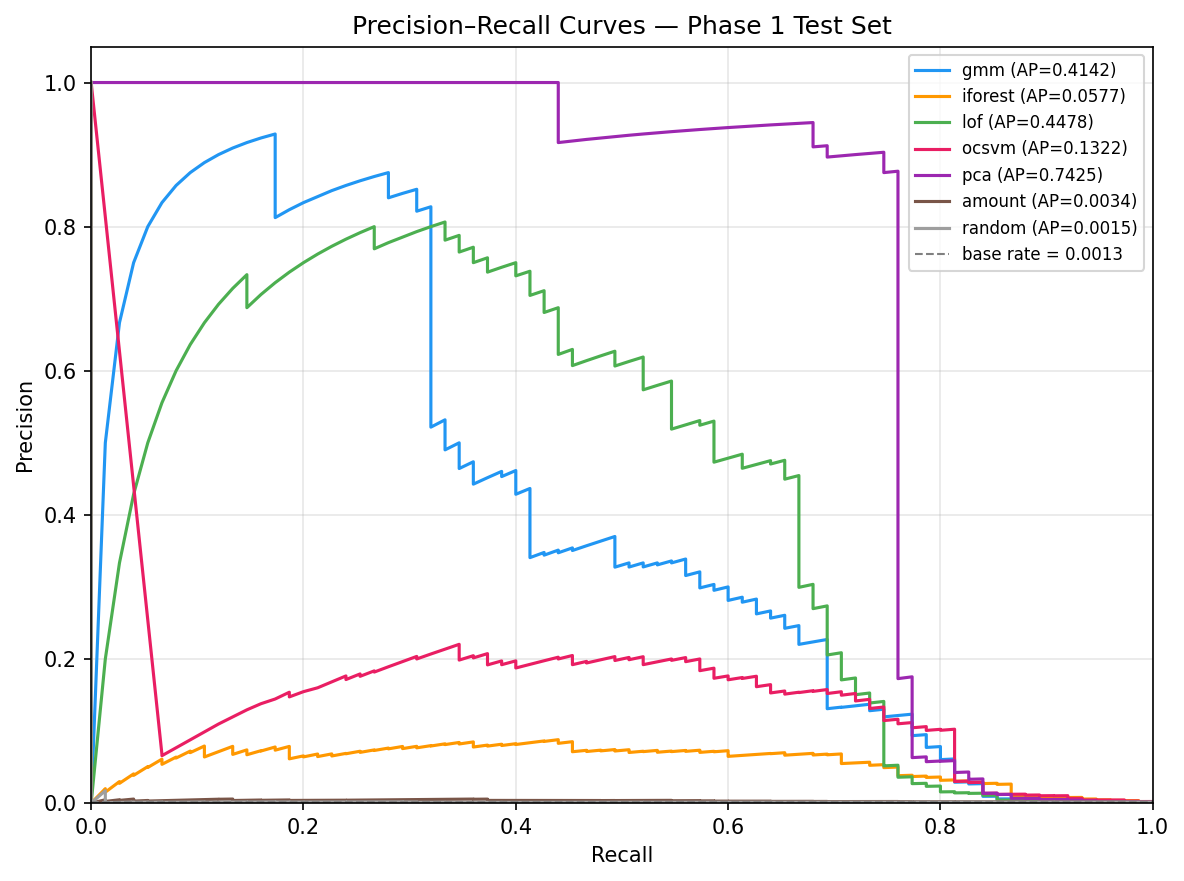
\includegraphics[width=0.85\linewidth]{results/figures/eval_pr_curves.png}
    \caption{Precision-Recall curves on the test set for all Phase~1 models.
    The dashed line is the fraud base rate ($\approx 0.132$\,\%).}
    \label{fig:pr}
\end{figure}


\subsection{Threshold Policy Results}
\label{sec:results:thresholds}

Table~\ref{tab:thresholds} summarises the FPR-budget threshold policies applied
to the test set for the top-performing PCA model.  All thresholds were derived
from the validation set and frozen before evaluation on test.

\begin{table}[htbp]
\centering
\caption{FPR-budget threshold results on the test set for PCA (best model).
Thresholds were derived from validation legitimate scores and frozen.}
\label{tab:thresholds}
\small
\begin{tabular}{l c c c c c c c}
\toprule
\textbf{Policy} & \textbf{Thresh.} & \textbf{Alerts} & \textbf{TP} &
\textbf{FP} & \textbf{Precision} & \textbf{Recall} & \textbf{F1} \\
\midrule
FPR$\leq$0.1\% & 0.5615 & 141 & 57 & 84  & 0.4043 & 0.7600 & 0.5278 \\
FPR$\leq$0.5\% & 0.1715 & 390 & 58 & 332 & 0.1487 & 0.7733 & 0.2495 \\
FPR$\leq$1.0\% & 0.0916 & 750 & 58 & 692 & 0.0773 & 0.7733 & 0.1406 \\
\bottomrule
\end{tabular}
\end{table}


\subsection{Cost Curve}
\label{sec:results:cost}

Figure~\ref{fig:cost} shows the expected cost per transaction at the optimal
threshold for each assumed cost ratio $r$ (missed fraud = $r \times$ false
alarm).  As $r$ increases, the optimal threshold decreases (more aggressive
flagging), trading more false alarms for fewer missed frauds.

\textbf{Important}: the cost ratio $r$ is an assumption.  These results show
how threshold selection depends on the business context, not a recommendation
for a specific operating point.

\begin{figure}[htbp]
    \centering
    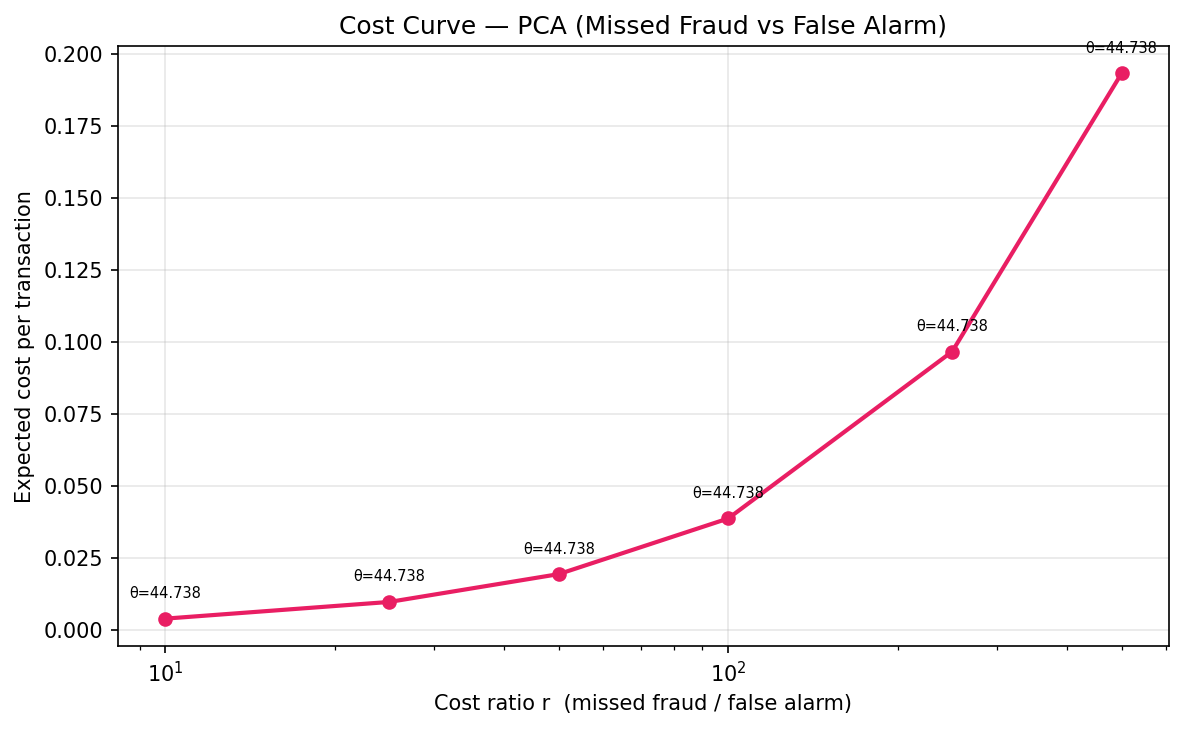
\includegraphics[width=0.75\linewidth]{results/figures/eval_cost_curve.png}
    \caption{Expected cost per transaction vs.\ cost ratio $r$.  The optimal
    threshold (annotated) shifts lower as missed-fraud cost increases.}
    \label{fig:cost}
\end{figure}


%%% ─── 9. Discussion & Limitations ──────────────────────────────────────────
\section{Discussion \& Limitations}

\subsection{Which model wins and why?}
PCA reconstruction error outperforms all other methods (PR-AUC \PRAUCTestPCA{}).
This is intuitive: the 28 V-features are PCA outputs from legitimate transactions,
so legitimate transactions are naturally well-reconstructed from a small number of
principal components. Fraud transactions, being drawn from a different distribution,
exhibit higher reconstruction residuals.

\subsection{Why does GMM underperform in validation?}
GMM validation PR-AUC (\PRAUCValGMM{}) is substantially lower than test
(\PRAUCTestGMM{}). With only \NFraudVal{} frauds in validation, the PR-AUC
estimate is highly variable (CI: [0.31, 0.54] on test). The GMM's component
selection via AIC/BIC on the validation split is thus unreliable. This
demonstrates the ``identify the gap'' result: GMM density scoring is sensitive
to the number of components, the covariance regularisation, and the number of
frauds available for threshold calibration.

\subsection{Where does Isolation Forest fail?}
Isolation Forest (PR-AUC \PRAUCTestIFOREST{}) performs near the random
reference. In high dimensions (31 features), random axis-aligned partitions
fail to isolate anomalies because the effective volume difference between
normal and anomalous regions vanishes --- a manifestation of the curse of
dimensionality.

\subsection{False-alert burden}
At FPR=0.5\%, the best model (PCA) would flag approximately 285 legitimate
transactions per 56,962 (0.5\%) to catch 58 of 75 frauds (77\%). A fraud
review team with capacity to investigate 285 cases per period captures 77\%
of fraud. Reducing to FPR=0.1\% cuts alerts to 57 but recall drops to 76\%.

\subsection{Threats to validity}
\begin{itemize}
  \item \textbf{Few test frauds (\NFraudTest{})}: Bootstrap CIs are wide;
        differences between LOF and GMM are not statistically significant.
  \item \textbf{PCA-anonymised features}: We cannot engineer domain-specific
        features or interpret which merchant categories drive fraud.
  \item \textbf{48-hour window}: Seasonal and weekly patterns are absent.
        The model may not generalise to different time periods.
  \item \textbf{Single dataset}: Results may not transfer to other card networks.
  \item \textbf{Assumed cost ratios}: Cost curve analysis assumes missed fraud
        costs 10--500$\times$ a false alarm; actual costs are bank-specific.
\end{itemize}

\textbf{Disclaimer}: This is a research prototype, not a production fraud system.

%%% ─── 10. Conclusion & Future Work ─────────────────────────────────────────
\section{Conclusion \& Future Work}

We compared five unsupervised anomaly-detection methods for credit card fraud
triage using the ULB dataset. PCA reconstruction error achieves the best
precision-recall performance (PR-AUC \PRAUCTestPCA{}) on the chronologically
held-out test set, outperforming GMM, LOF, OC-SVM, and Isolation Forest.
The GMM instability study confirms that Gaussian mixture density scoring is
sensitive to dimensionality, regularisation, and limited fraud events for
validation. Future work (Phase 2) will compare a deep undercomplete autoencoder
reconstruction scorer, which is hypothesised to learn a more expressive
non-linear manifold of legitimate transactions.

%%% ─── 11. Individual Contributions ─────────────────────────────────────────
\section{Individual Contributions}

\begin{itemize}
  \item \textbf{Kushal Sarkar}: Project scaffold, data pipeline, metrics module,
        integration, final comparison, report assembly.
  \item \textbf{Prachee Dhar}: Literature review ($\geq$12 verified references),
        EDA (duplicates, imbalance, KS drift, Gaussianity checks).
  \item \textbf{Apoorva Choudhary}: Feature engineering, GMM grid search
        (covariance type $\times$ K), AIC/BIC analysis, EM theory, instability study.
  \item \textbf{Vani Rudra}: Classical baselines (PCA, Isolation Forest, OC-SVM, LOF),
        hyperparameter sweeps, theory sections.
  \item \textbf{Krishna Pramod Dubale}: Evaluation toolkit, bootstrap CIs,
        threshold policies, cost curves, master comparison table.
\end{itemize}

%%% ─── References ─────────────────────────────────────────────────────────────
\bibliographystyle{IEEEtran}
\bibliography{refs}

\end{document}
